
% \usepackage[utf8]{inputenc} % allow utf-8 input
% \usepackage[T1]{fontenc}    % use 8-bit T1 fonts
% \usepackage[hidelinks]{hyperref}% hyperlinks
% \usepackage{url}            % simple URL typesetting
% \usepackage{booktabs}       % professional-quality tables
% \usepackage{amsfonts}       % blackboard math symbols
% \usepackage{nicefrac}       % compact symbols for 1/2, etc.
% \usepackage{microtype}      % microtypography
% \usepackage{xcolor}         % colors

% \usepackage{lipsum}

% \newcommand\blfootnote[1]{%
%   \begingroup
%   \renewcommand\thefootnote{}\footnote{#1}%
%   \addtocounter{footnote}{-1}%
%   \endgroup
% }



% \title{Conformal Off-Policy Prediction in Contextual Bandits}


% The \author macro works with any number of authors. There are two commands
% used to separate the names and addresses of multiple authors: \And and \AND.
%
% Using \And between authors leaves it to LaTeX to determine where to break the
% lines. Using \AND forces a line break at that point. So, if LaTeX puts 3 of 4
% authors names on the first line, and the last on the second line, try using
% \AND instead of \And before the third author name.

% \author[1]{Muhammad Faaiz Taufiq*} 
% \author[2]{Jean-Fran\c cois Ton*} 
% \author[1]{Rob Cornish} 
% \author[1]{Yee Whye Teh} 
% \author[1]{Arnaud Doucet} 

% \affil[1]{Department of Statistics, University of Oxford}
% \affil[2]{ByteDance Research}

% \author{%
%   Muhammad Faaiz Taufiq* \\
%   Department of Statistics\\
%   University of Oxford\\
%   % examples of more authors
%    \And
%    Jean-Francois Ton*$^\dagger$ \\
%    AI-Lab-Research\\
%    Bytedance AI Lab \\
%    \AND
%    Rob Cornish \\
%    Department of Statistics \\
%    University of Oxford\\
%    \And
%    Yee Whye Teh \\
%    Department of Statistics \\
%    University of Oxford\\
%    \And
%    Arnaud Doucet \\
%    Department of Statistics \\
%    University of Oxford\\
% }



\begin{abstract}
  Most off-policy evaluation methods for contextual bandits have focused on the expected outcome of a policy, which is estimated via methods that at best provide only asymptotic guarantees. However, in many applications, the expectation may not be the best measure of performance as it does not capture the variability of the outcome. In addition, particularly in safety-critical settings, stronger guarantees than asymptotic correctness may be required. To address these limitations, we consider a novel application of conformal prediction to contextual bandits. Given data collected under a behavioral policy, we propose \emph{conformal off-policy prediction} (COPP), which can output reliable predictive intervals for the outcome under a new target policy. We provide theoretical finite-sample guarantees without making any additional assumptions beyond the standard contextual bandit setup, and empirically demonstrate the utility of COPP compared with existing methods on synthetic and real-world data. 
  % \blfootnote{$^*$Denotes equal contribution, where ordering was determined through coin flip. Corresponding authors \texttt{muhammad.taufiq@stats.ox.ac.uk} and \texttt{jeanfrancois@bytedance.com}.
%   \blfootnote{$\dagger$ Work primarily done at the University of Oxford and finished at Bytedance.}
\end{abstract}

\section{Introduction}
% Often in safety-critical environments such as healthcare, we cannot afford to implement new policies, without reliably evaluating the effectiveness/safety of the policies. In such situations, we must resort to using available observational data to infer outcomes under a new target policy which has not been implemented in the real world. This is known as off-policy evaluation. 


% \R{In domains such as healthcare or recommendation systems, understanding all the possible outcomes is at the core of safe and informed decision making.} Due to ethical or financial constraints, we can often not implement new policies $\pi^*$, without first reliably evaluating its effectiveness and safety. In such cases we have to rely on observational data, which has been collected under a different policy $\pi^b$. Using this data to evaluate a policy $\pi^*$ is known as off-policy evaluation (OPE) and helps us assess $\pi^*$ without having to deploy it.
% % which can be both costly and risky. we use the same formulationas in Romano et al. (2019), i.
% % Hence it is crucial to determine the most likely outcomes under a new policy in a reliable manner.


Before deploying a decision-making policy to production, it is usually important to understand the plausible range of outcomes that it may produce.
However, due to resource or ethical constraints, it is often not possible to obtain this understanding by testing the policy directly in the real-world.
In such cases we have to rely on observational data collected under a different policy than the target.
Using this observational data to evaluate the target policy is known as off-policy evaluation (OPE).% and helps us assess $\pi^*$ without having to deploy it.


% policies $\pi^*$, without first reliably evaluating its effectiveness and safety. In such cases we have to rely on observational data, which has been collected under a different policy $\pi^b$. Using this data to evaluate a policy $\pi^*$ is known as off-policy evaluation (OPE) and helps us assess $\pi^*$ without having to deploy it.

% To make safe and informed decisions, it is important to understand the range of plausible outcomes that may occur under the different choices available.


% Due to the tremendous increase in data availability over the years, we often find ourselves in situations where we have an abundance of observational data, i.e. data which has been collected under a certain unknown behaviour policy $\pi^b$ but want to infer outcomes \textit{as if} the data was collected under $\pi^*$. In cases, where a new policy $\pi^*$ is expensive or unethical to implement, we have to rely on the observational data and perform off-policy evaluations (OPE) of $\pi^*$ in order to determine whether the new policy can be safely implemented in the real world. Hence it is crucial to be able to determine the most likely outcomes under a new policy in a reliable manner.
% Due to the popularity of concentration inequalities \cite{concentrationineq} computing bounds on the expectation becomes feasible. 
% 1. Doesn't take into account any notions of variance. 
% 2. Can be highly prone to outliers, especially, when the size of data is small. 
% -> Therefore, often in safety-critical settings, like econometrics, metrics such as VaR (Value at Risk) are used as they are better representations of potential risk. 
% -> instead, in safety-critical settings, where one might be concerned with minimizing potential risk, the distribution of the outcome itself might be more informative. 

Traditionally, most techniques for OPE in contextual bandits focus on evaluating policies based on their \textbf{expected} outcomes; see e.g., \cite{uncertainty5, adaptive-ope, uncertainty2, uncertainty3, uncertainty4, doubly-robust}.
However, this can be problematic as methods that are only concerned with the average outcome do not take into account any notions of variance, for example. Therefore, in risk-sensitive settings such as econometrics, where we want to minimize the potential risks, metrics such as CVaR (Conditional Value at Risk) might be more appropriate \citep{keramati2020being}. Additionally, when only small sample sizes of observational data are available, the average outcomes under finite data can be misleading, as they are prone to outliers and hence, metrics such as medians or quantiles are more robust in these scenarios \citep{altschuler2019best}.

% and hence, predictive bounds based on the outcome distribution instead of the average are more informative. 
% Hence, in high stake settings such as healthcare where medical practitioner are more concerned with minimizing potential risk, knowing high probability bounds of possible outcomes of a new policy is extremely useful, as it allows them to make better informed decisions. In recommendation systems where a vast majority of the data are be outliers, methodologies that focus on the average outcome become misleading and uninformative. 
%  In addition, due to the finite data regime these methods are very susceptible to outliers [refs].
\begin{figure}
     \centering
     \begin{subfigure}[t]{0.5\textwidth}
         \centering
         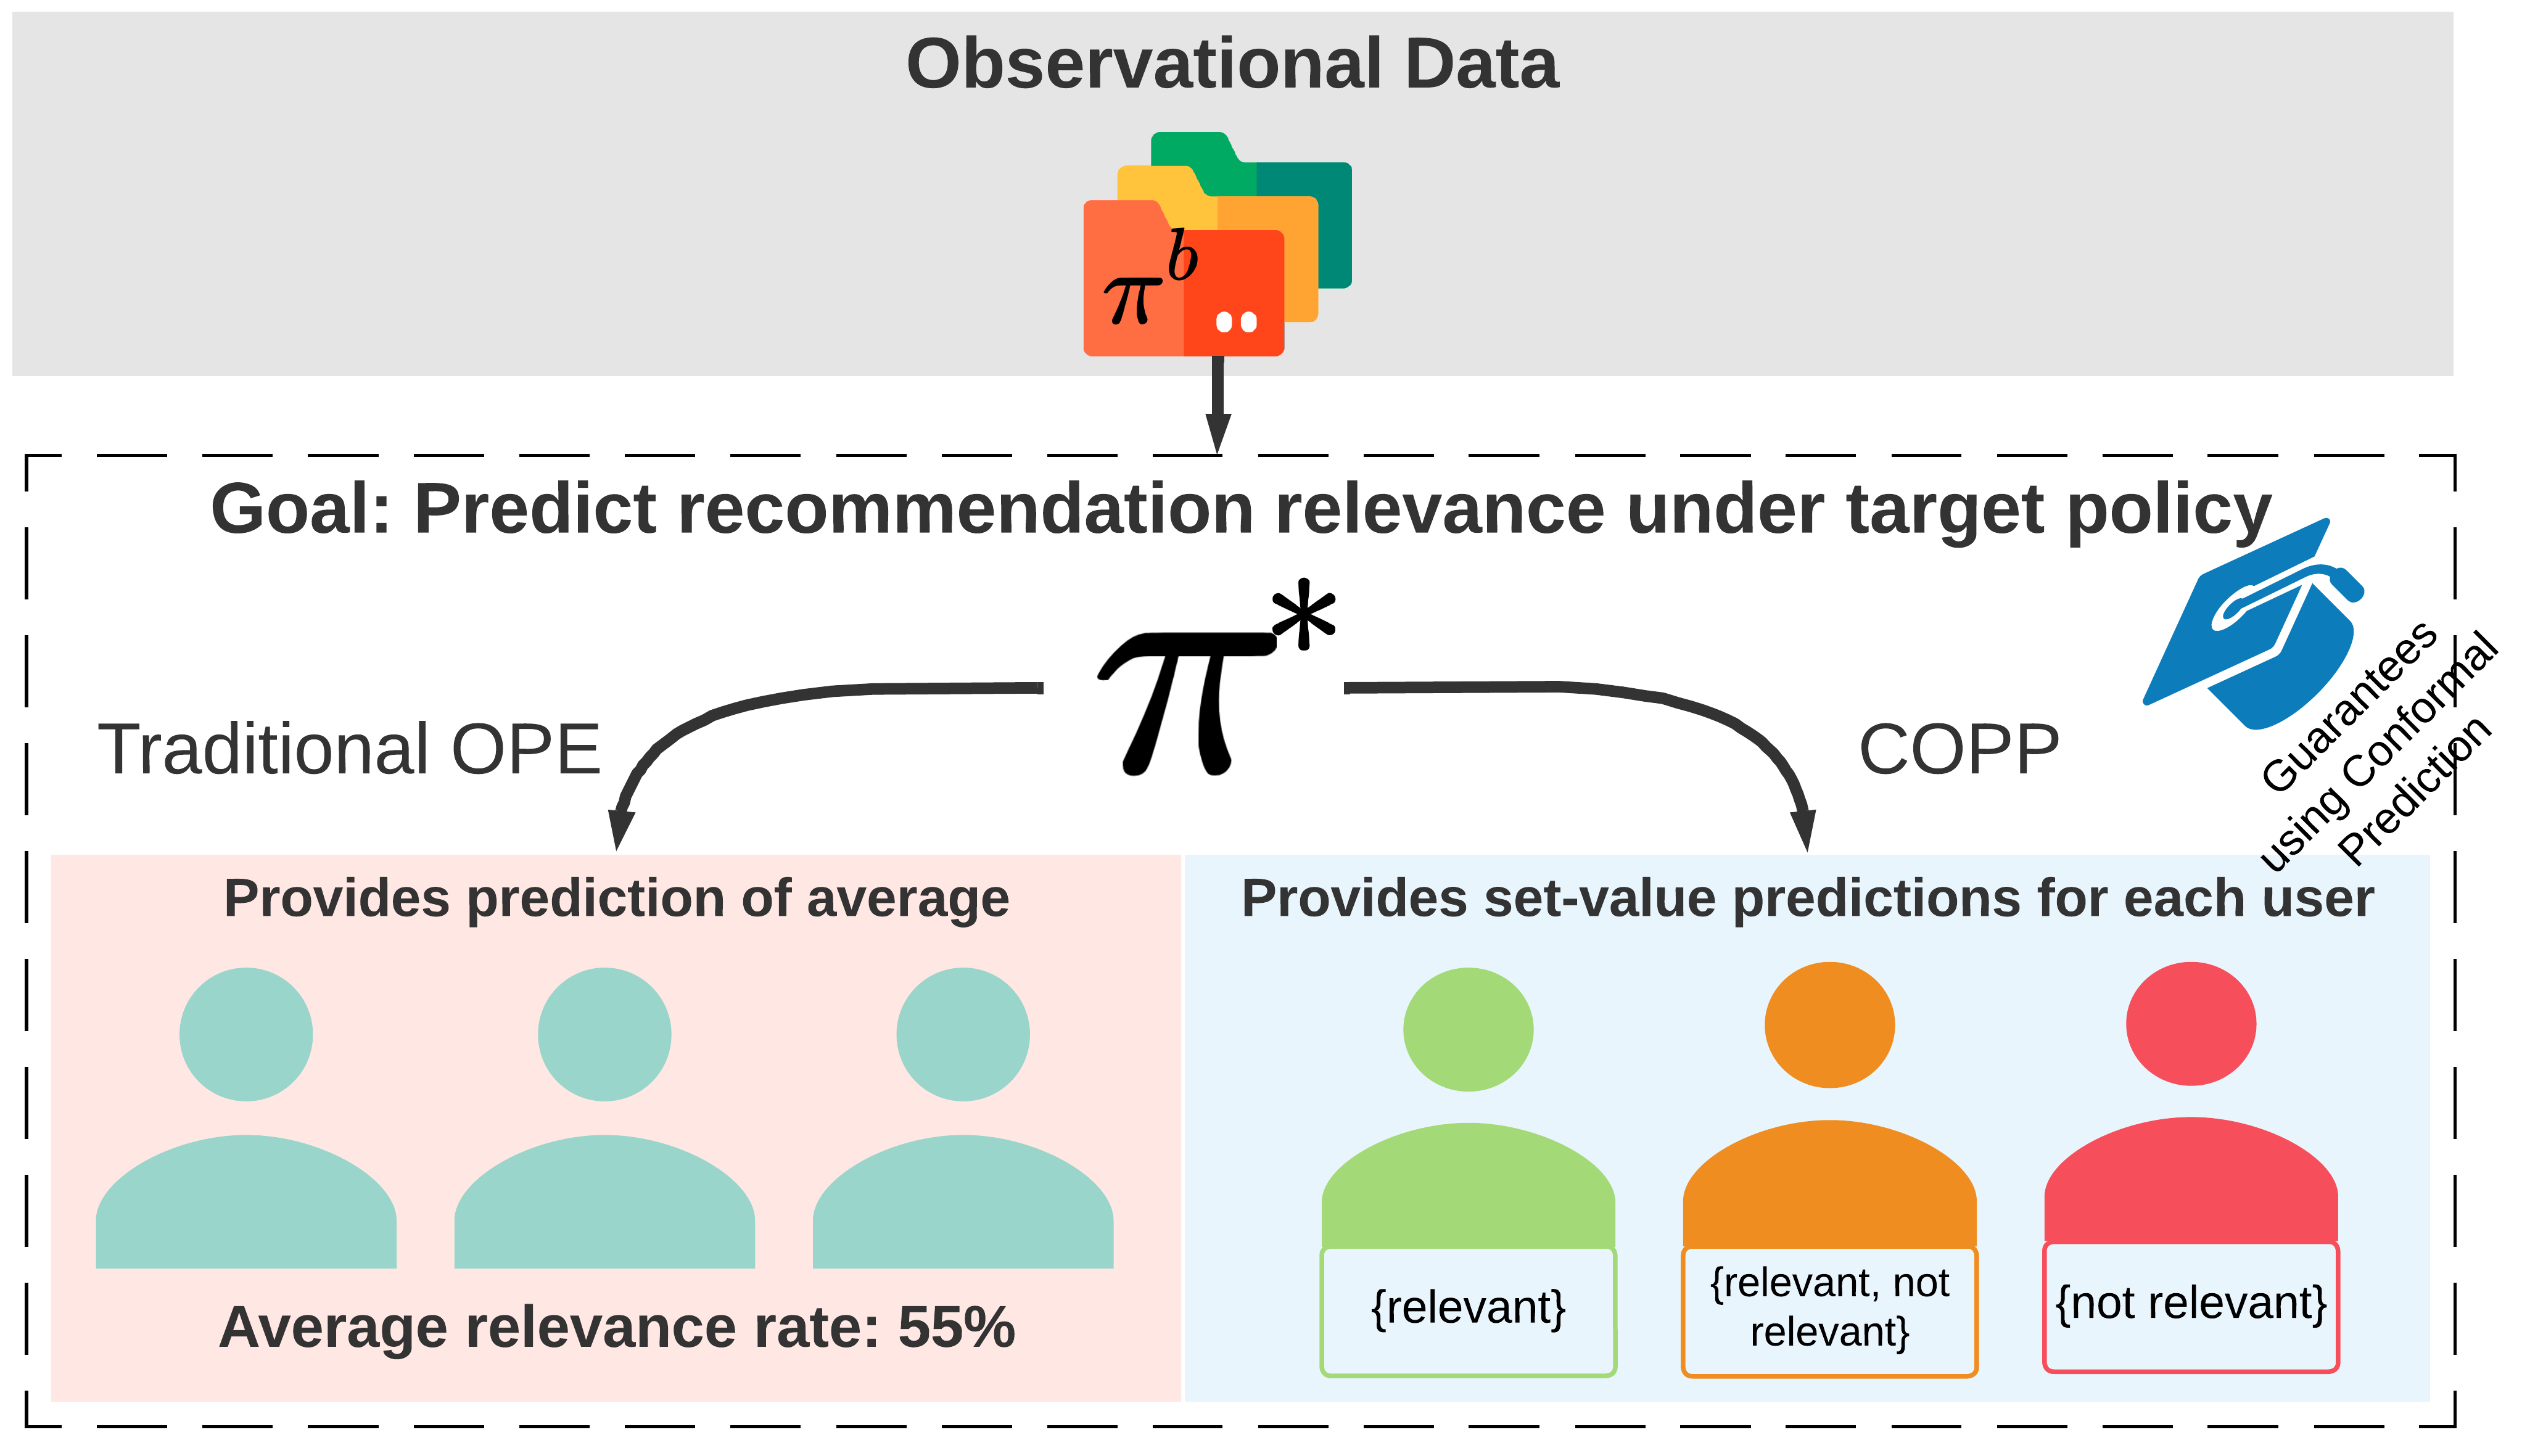
\includegraphics[height=1.85in]{figures/copp/COPP7.png}
        %  \subcaption{Conformal Off-Policy Prediction compared to standard off-policy evaluation methods.}
        %  \label{fig:copp}
     \end{subfigure}%\hspace{0.8cm}%
     \begin{subfigure}[t]{0.5\textwidth}
         \centering
         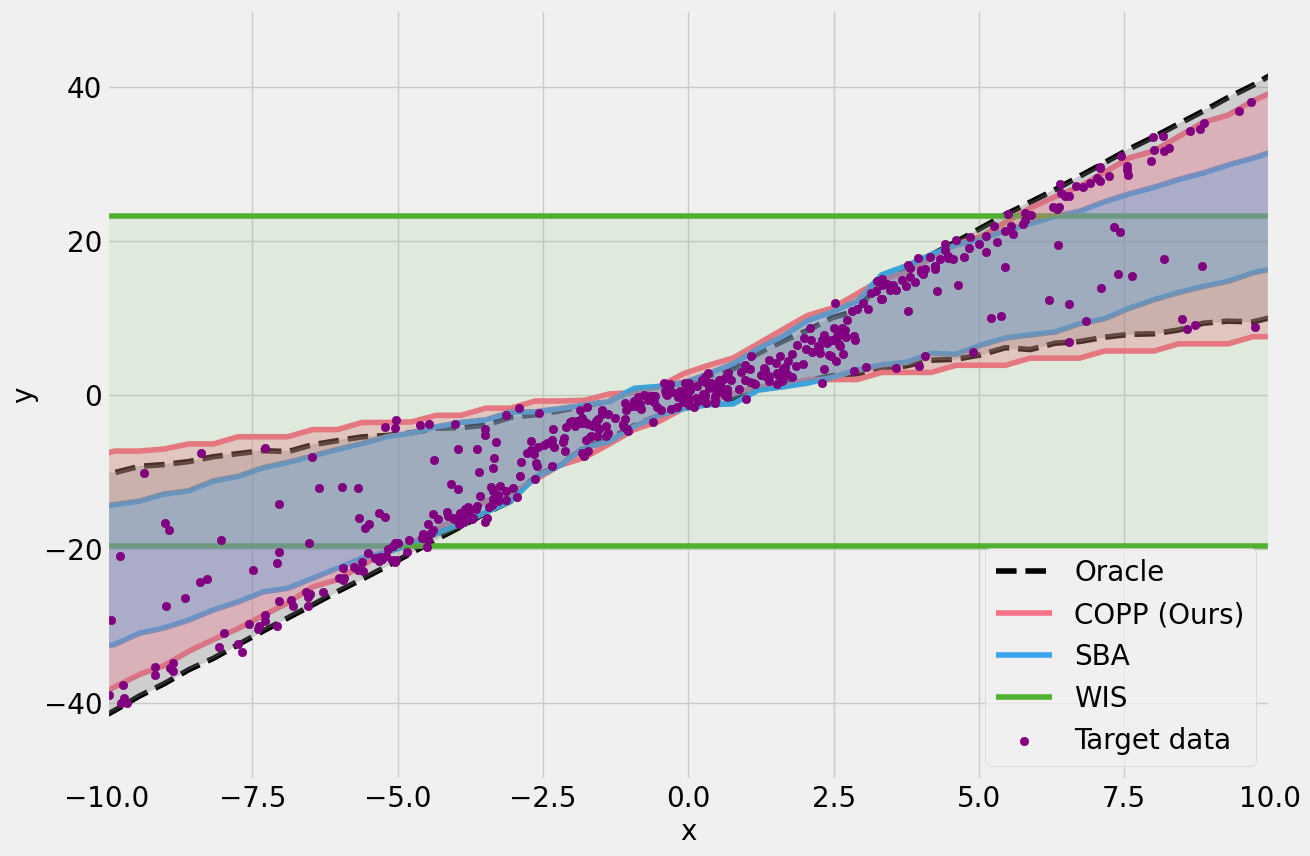
\includegraphics[height=1.85in]{figures/copp/cis-updated.png}
        %  \subcaption{$90\%$ predictive intervals for $Y$ as a function of $X$ for COPP, competing methods and the oracle.}
        %  \label{fig:cis-updated}
     \end{subfigure}

    \caption{\textbf{Left (a):} Conformal Off-Policy Prediction against standard off-policy evaluation methods. \textbf{Right (b):} $90\%$ predictive intervals for $Y$ against $X$ for COPP, competing methods and the oracle.}\label{fig:copp}
    % \label{fig:three graphs}
\end{figure}


% \begin{figure}
%     \centering
%     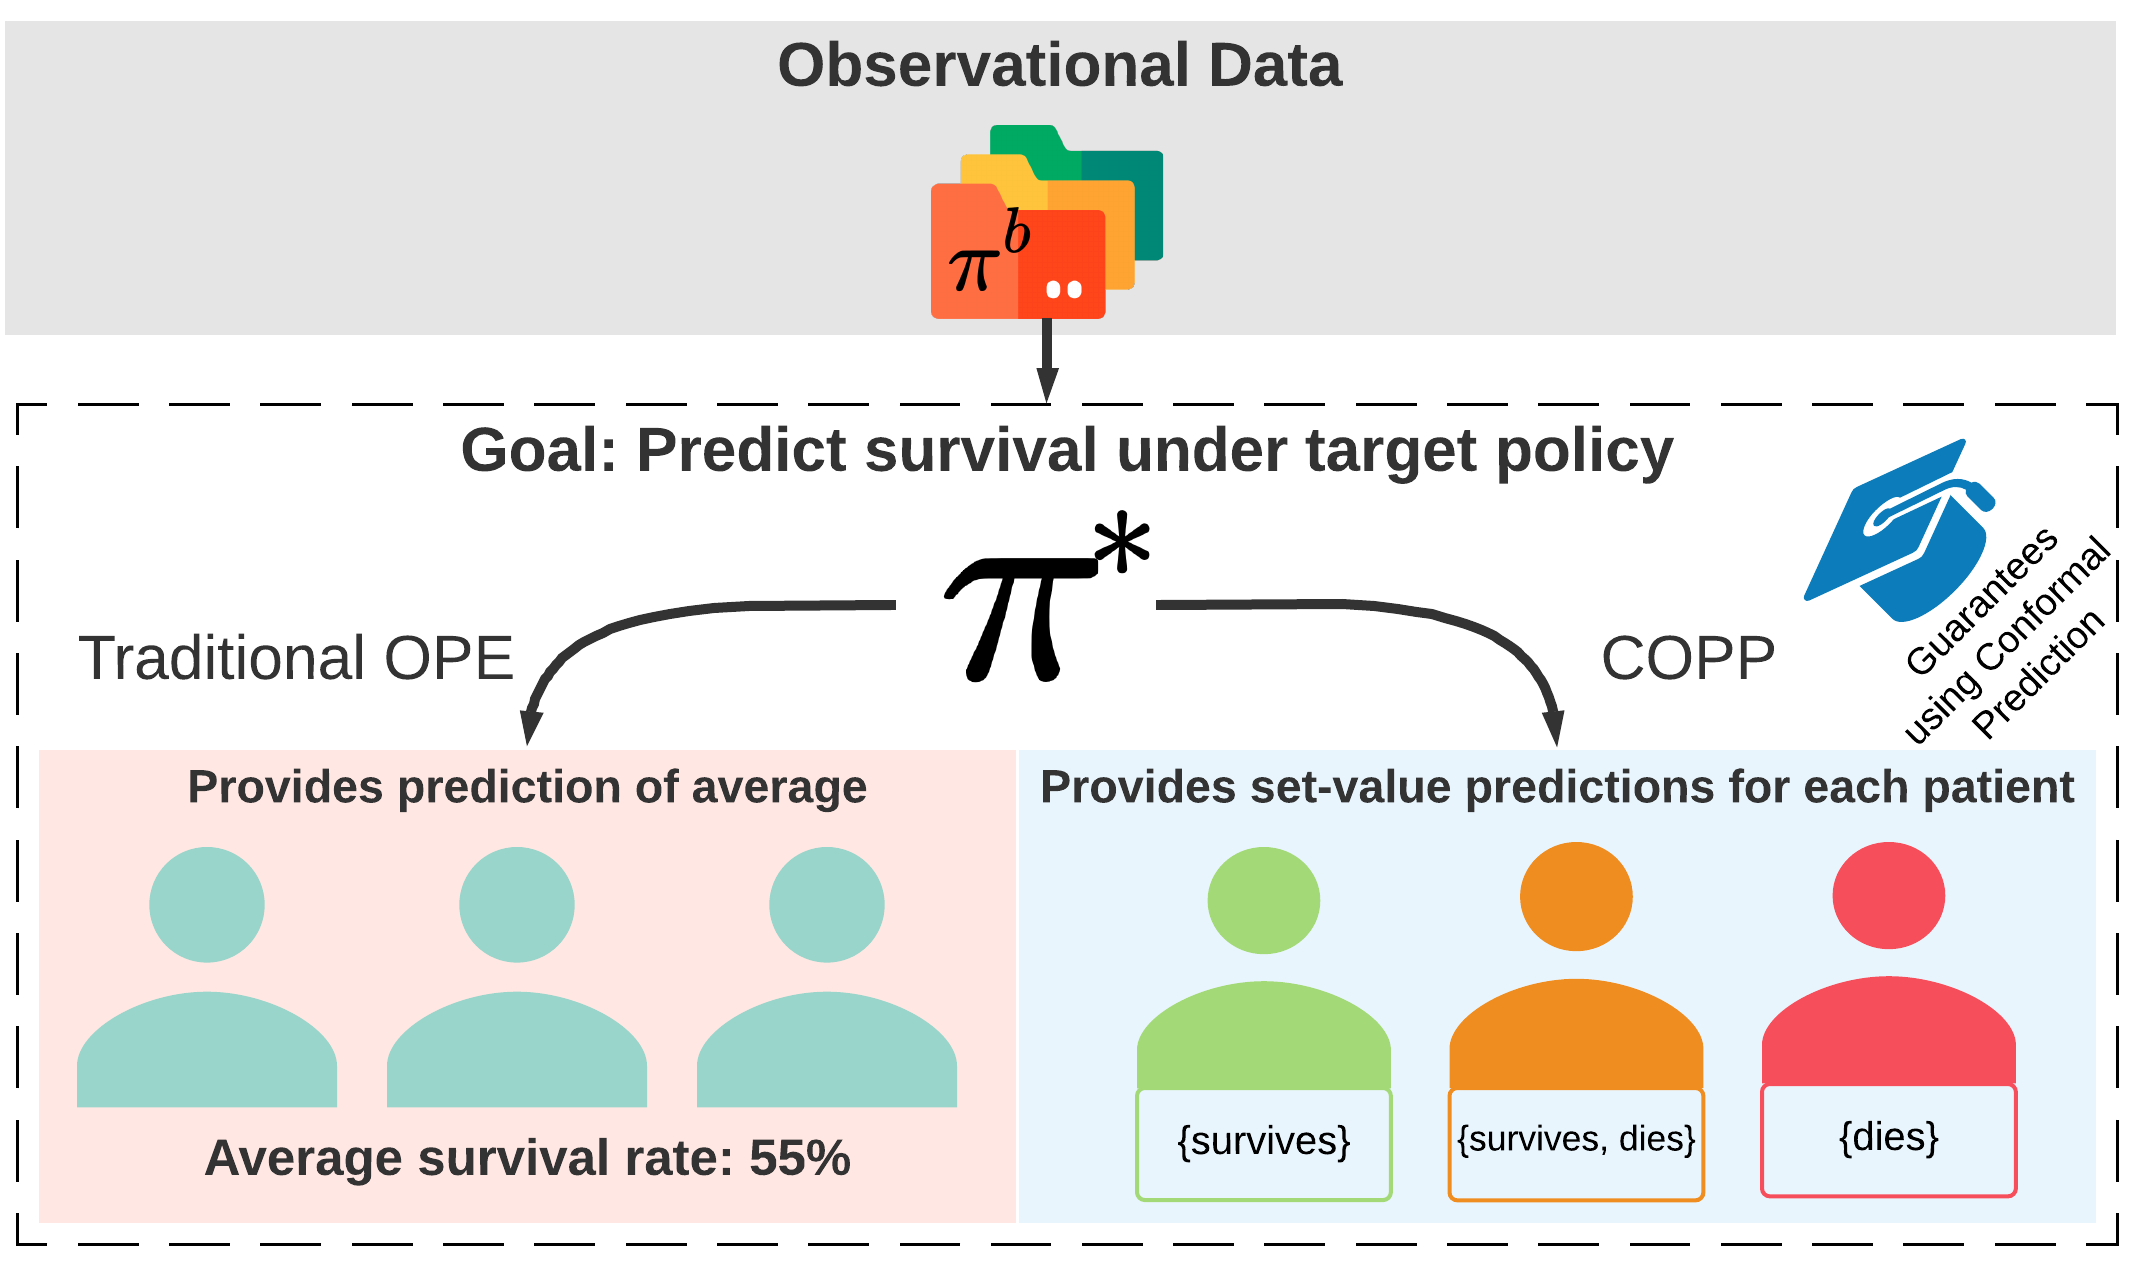
\includegraphics[width=0.5\columnwidth]{figures/copp/COPP5.png}
%     \caption{Illustration of Conformal Off-Policy Prediction compared to standard off-policy evaluation methods.}
%     \label{fig:copp}
% \end{figure}
Notable exceptions in the OPE literature are \cite{risk-assessment, chandak2021universal}. Instead of estimating bounds on the expected outcomes, \cite{risk-assessment, chandak2021universal} establish finite-sample bounds for a general class of metrics (e.g., Mean, CVaR, CDF) on the outcome. Their methods can be used to estimate quantiles of the outcomes under the target policy and are therefore robust to outliers. However, the resulting bounds do not depend on the covariates $X$ (not adaptive w.r.t. $X$). This can lead to overly conservative intervals, as we will show in our experiments and can become uninformative when the data are heteroscedastic (see Fig. \ref{fig:copp}b).

%  Instead of investigating the bounds on the expected outcomes, \cite{risk-assessment, chandak2021universal} propose an off-policy assessment in contextual bandits setting to construct bounds that enjoy finite-sample guarantees. In particular, the authors aim to construct estimators for the CDF of the return and hence are able determine quantities such as the median or the $95\%$ quantiles of the rewards, which as mentioned above, are crucial for robustness and uncertainty quantification. Note that the CDF estimators proposed by \cite{risk-assessment, chandak2021universal} do not depend on the specific $X$, and as a result the bounds obtained are not adaptive w.r.t. $X$. 

% Furthermore, while the distributional perspective without CDFs has been explored in the context of Reinforcement Learning \cite{distributional-rl}, to the best of our knowledge they do not provide any finite-sample guarantees.

% In this paper, we propose Conformal Off-Policy Prediction (COPP), a novel algorithm based on Conformal Prediction (CP) that produces predictive interval/sets for off-policy outcomes in contextual bandits (see Fig.\ref{fig:copp}a).
% To the best of our knowledge, this is the first method to obtain predictive intervals in the off-policy setting that enjoys both finite-sample theoretical guarantees and adaptivity w.r.t.\ the covariates $X$.
% % We achieve this by using conformal prediction (CP), a distribution-free uncertainty quantification method pioneered by \cite{vovk2005algorithmic}.
% %and can be used on top of any black-box model.
% Unlike previous work, which assumed a deterministic target and discrete action space, our approach is valid for stochastic target policies and continuous action spaces, which lifts the restriction of previous related work to deterministic targets and discrete actions.
% %, our approach can be applied to both deterministic and stochastic target policies, as well as discrete and continuous actions spaces.}

% In this paper, we propose Conformal Off-Policy Prediction (COPP), a novel algorithm for constructing predictive interval/sets for off-policy outcomes in contextual bandits (see Fig.\ref{fig:copp}a).
In this paper, we propose Conformal Off-Policy Prediction (COPP), a novel algorithm that uses Conformal Prediction (CP) \citep{vovk2005algorithmic} to construct predictive interval/sets for outcomes in contextual bandits (see Fig.\ref{fig:copp}a) using an observational dataset.
COPP enjoys both finite-sample theoretical guarantees and adaptivity w.r.t.\ the covariates $X$, and, to the best of our knowledge, is the first such method based on CP that can be applied to stochastic policies and continuous action spaces.
% To the best of our knowledge, COPP is the first such method that enjoys both finite-sample theoretical guarantees and adaptivity w.r.t.\ the covariates $X$.
% Unlike earlier work, our approach can be applied to stochastic policies and continuous action spaces.
% Unlike related work involving CP, our approach can be applied to both deterministic and stochastic target policies
% We achieve this via conformal prediction (CP), a distribution-free uncertainty quantification method pioneered by \cite{vovk2005algorithmic}.
%and can be used on top of any black-box model.

% % {\color{red} Our approach also applies to stochastic target policies which have not been considered by previous work on CP.}
% % Most importantly, CP produces predictive intervals that have finite-sample coverage guarantees, i.e. the interval will contain the ground truth outcome with a certain user pre-specified threshold $\alpha$.
% Our paper also makes the following additional contributions.
% (i)
% % Our approach is widely applicable: previous work involving CP has been limited to deterministic policies and discrete action spaces, while our method applies also for discrete and continuous.
% % Our approach is more widely applicable than previous work involving CP, and can be used for stochastic policies and continuous action spaces.
% % Our approach lifts restrictions present in related work involving CP, 
% % \R{Unlike related work involving CP, our approach can be applied to both deterministic and stochastic target policies, as well as discrete and continuous actions spaces.}
% \R{Our approach remains valid for stochastic target policies and continuous action spaces, which lifts the restriction of previous related work to deterministic targets and discrete actions.} %, our approach can be applied to both deterministic and stochastic target policies, as well as discrete and continuous actions spaces.}
% % \R{Unlike related work involving CP, our approach can be applied to both deterministic and stochastic target policies}
% % (ii) We provide theoretical guarantees for COPP, including finite-sample guarantees on marginal coverage and asymptotic guarantees on conditional coverage.
% (ii) We provide a theoretical analysis of COPP, including finite-sample guarantees on marginal coverage and asymptotic guarantees on conditional coverage.
% (iii) We show empirically that COPP outperforms standard methods in terms of coverage and predictive interval width when assessing new policies. 

% {\color{red} Our approach also applies to stochastic target policies which have not been considered by previous work on CP.}
% Most importantly, CP produces predictive intervals that have finite-sample coverage guarantees, i.e. the interval will contain the ground truth outcome with a certain user pre-specified threshold $\alpha$.
In summary, our contributions are: 
% (i) We adapt results from the CP literature to construct predictive intervals for the outcome $Y$ under a new policy which are adaptive w.r.t.\ $X$.
% (i) We construct valid predictive intervals for bandit outcomes that applies in more general settings (stochastic policies and continuous actions) than previous work.
(i) We propose an application of CP to construct predictive intervals for bandit outcomes that is more general (applies to stochastic policies and continuous actions) than previous work.
% Our approach is widely applicable: previous work involving CP has been limited to deterministic policies and discrete action spaces, while our method applies also for discrete and continuous.
% Our approach is more widely applicable than previous work involving CP, and can be used for stochastic policies and continuous action spaces.
% Our approach lifts restrictions present in related work involving CP, 
% \R{Unlike related work involving CP, our approach can be applied to both deterministic and stochastic target policies, as well as discrete and continuous actions spaces.}
% \R{Our approach avoids various restrictions of earlier work, being valid for stochastic target policies and continuous action spaces.} %, our approach can be applied to both deterministic and stochastic target policies, as well as discrete and continuous actions spaces.}
% \R{Unlike related work involving CP, our approach can be applied to both deterministic and stochastic target policies}
(ii) We provide theoretical guarantees for COPP, including finite-sample guarantees on marginal coverage and asymptotic guarantees on conditional coverage.
(iii) We show empirically that COPP outperforms standard methods in terms of coverage and predictive interval width when assessing new policies. 

\subsection{Problem Setup}\label{sec:problem_setup}

\begin{comment}
% \begin{wrapfigure}{r}{0.22\textwidth}
\begin{figure}
    \centering
    \includegraphics[width=0.15\textwidth]{diagram1.pdf}
    \caption{Causal graph of our problem setup. The action $A$ is shaded to illustrate that we are ``integrating out'' the effect of the actions through the policy when predicting $Y$ from $X$.}
    \label{fig:OPE_conformal}
\end{figure}
% \end{wrapfigure}
\end{comment}
Let $\mathcal{X}$ be the covariate space (e.g., user  data), $\mathcal{A}$ the action space (e.g., recommended items) and $\mathcal{Y}$ the outcome space (e.g., relevance to the user).
We allow both $\mathcal{A}$ and $\mathcal{Y}$ to be either discrete or continuous.
In our setting, we are given logged observational data $\mathcal{D}_{obs}=\{x_i, a_i, y_i \}_{i=1}^{n_{obs}}$ where actions are sampled from a behavioural policy $\pi^{b}$, i.e. $A \mid x \sim \pi^{b}(\cdot\mid x)$ and $Y \mid x,a \sim P(\cdot \mid x, a)$. We assume that we do not suffer from unmeasured confounding. At test time, we are given a state $x^{test}$ and a new policy $\pi^*$. While $\pi^{b}$ may be unknown, we assume the target policy $\pi^*$ to be known.
% \begin{comment}
% \begin{align*}
%     \text{Standard OPE} \qquad & \mathbb{E}_{(X, Y) \sim P^{\pi^*}_{X,Y}}[Y] \\
%     \text{Huang} \qquad & \mathbb{E}_{(X, Y) \sim P^{{\pi^*}}_{X,Y}} [\varphi(Y)], \varphi \in \Phi \\
%     \text{Us} \qquad &  \hat{C} \text{ s.t. } 1- \alpha \hspace{-0.05cm}\leq  \tarprob(Y \in \hat{C}(X)) \hspace{-0.05cm}\leq 1- \alpha + o_{n_{obs}}(1)
% \end{align*}
% \end{comment}
% \begin{comment}
% % Properties of interest: 1. adaptivity w.r.t x 2. capturing of the variability in outcomes 3. finite sample guarantees. 
% In this paper we aim to construct intervals $\hat{C}(x)$ on the outcome $Y$ which are (i) dependent on $x$, (ii) capture the variability in outcomes $Y$ and (iii) provide finite sample guarantees. Current explored methodologies lack at least one of these properties (see Table [] in section). 
% In particular, property (ii) can be achieved if $\hat{C}(x)$ captures the true outcome $Y$ with any pre-specified probability $1-\alpha$. One way to express this formally is as follows:
% \begin{align}
%      \hspace{-0.24cm}1- \alpha \hspace{-0.05cm}\leq  \tarprob(Y \in \hat{C}(X)) \hspace{-0.05cm}\leq 1- \alpha + o_{n_{obs}}(1) \label{guarantee}
% \end{align}
% where $n_{obs}$ is the size of available observational data and $P^{\pi^*}_{X,Y}$ is the joint distribution of $(X,Y)$ under target policy $\pi^*$. The probability is taken over the joint distribution of $(X, Y)$, meaning that the interval holds in the marginal sense in $X$ (marginal coverage) and not for a given $X=x$ (conditional coverage). In Section \ref{sec:cond_cov}, we provide additional regularity conditions under which not only marginal but also conditional coverage holds. Moreover, given that we are interested in the outcomes under $\pi^*$, the intervals $\hat{C}(x)$ are not conditioned on a specific $a$, but rather on $\pi^*$. 
% In this paper, we construct $\hat{C}(x)$ which satisfies \eqref{guarantee} along with the properties (i)-(iii), using the CP framework, which we will introduce in the following section. 
% % Our proposed methodology uses CP to construct $\hat{C}(x)$ and provides finite-sample coverage guarantees on the outcomes $Y$ given a current state $X$ and a target policy $\pi^* (a\mid x)$, hence allowing us to be confident in terms of the outcomes, when deploying a new policy.
% % \textbf{Explanation of the objective: } 
% % The :
% % Standard OPE & \mathbb{E}_{(X, Y) \sim P^{\pi^*}_{X,Y}}[Y] & (1) x (2) x (3) \tick
% % Huang et al & \mathbb{E}_{(X, Y) \sim P^{\pi^*}_{X,Y}}[\phi(Y]) & (1) \tick 2(x) (3) \tick
% % In this setting the quantities of interests in the current literature are:
% % \begin{align*}
% %     \text{Standard OPE} \qquad & \mathbb{E}_{(X, Y) \sim P^{\pi^*}_{X,Y}}[Y] \\
% %     \text{Huang} \qquad & \mathbb{E}_{(X, Y) \sim P^{{\pi^*}}_{X,Y}} [\varphi(Y)], \varphi \in \Phi
% % \end{align*}
% % However, none of these objectives take into account take into account both the finite sample guarantees and the adaptivity w.r.t. $x$. Hence we propose to construct predictive intervals on the outcomes which are adaptive w.r.t. $x$, and provide finite sample guarantees
% In standard OPE literature the main objective is to estimate $\mathbbm{E}[sth]$
% \end{comment}
% \textbf{Our goal} is to obtain predictive intervals/sets, $\hat{C}(x^{test})$, for a given $\alpha \in (0,1)$, which satisfy:
% \begin{align}
% \text{$P_{Y(a)}(y \mid X = x)$ for each $a$} \\
% \text{$C_a$ such that $\mathbb{P}(Y(a) \in C_a(X) \mid X = x) \geq 1 - \alpha$, for each $a$} \\
% \text{$C_a$ such that $\mathbb{P}(Y(a) \in C(X)) \geq 1 - \alpha$ for each $a$}
% \end{align}
% \begin{align}
%      \hspace{-0.24cm}1- \alpha \hspace{-0.05cm}\leq  \tarprob(Y \in \hat{C}(X)) \hspace{-0.05cm}\leq 1- \alpha + o_{n_{obs}}(1) \label{guarantee}
% \end{align}
% where $n_{obs}$ is the size of available observational data and $P^{\pi^*}_{X,Y}$ is the joint distribution of $(X,Y)$ under target policy $\pi^*$. Note that the probability is taken over the joint distribution of $(X, Y)$, meaning that the interval holds in the marginal sense in $X$ (marginal coverage) and not for a given $X=x$ (conditional coverage).  In Section \ref{sec:cond_cov}, we provide additional regularity conditions under which not only marginal but also conditional coverage holds.
% % The challenges in this case are to account for the shift in policy and obtain guarantees on the predictive interval $\hat{C}(X)$.
% To this end, we will use the CP framework to construct predictive intervals in order to assess a new policy. Our proposed methodology provides theoretical coverage guarantees on the outcome $Y$ given a current state $X$ and a target policy $\pi^* (a\mid x)$, hence allowing us to be confident in terms of the outcomes, when deploying a new policy.
% Huang et al.\ obtain a method for obtaining a richer evaluation of a given policy.
% Specifically, they estimate the $\varphi(p^{\pi^\ast}_{X,Y})$ for a more general class of functions $\varphi$ than just the expectation operator.
% While this allows for a much richer understanding of $\pi^\ast$, its expressiveness is still in some respects limited, as is clear from the fact that it does not depend on $X$, but only on $P_{X,Y}^{\pi^\ast}$.
% 
% The guarantees they get are usually only asymptotic, meaning that they approximate this quantity with 

% Existing methods focus on evaluating $\mathbb{E}_{(X, Y)\sim P^{\pi^*}_{X,Y}}[Y]$.
% This is useful for comparing two policies directly because it is just a single number, but does not provide a rich understanding of the behaviour of the policy on a per item basis.

% In this work, we present a method that avoids some of these shortcomings.
% Specifically, we construct a set-valued function $\hat{C}(x)$ that takes as input a covariate and outputs a \emph{subset} of $\mathcal{Y}$ rather than just a single point.
% This subset is guaranteed to contain the true value of $Y$ with a certain probability.
% Specifically, we obtain the guarantee:
% \[
% \tarprob(Y \in \hat{C}(X)) \geq 1 - \alpha.
% \]
% Moreover, we will show this guarantee holds for our method regardless of any distributional assumptions on $X$ and $Y$, and regardless of the size of the data we have available to us.

We consider the task of rigorously quantifying the performance of $\pi^*$ without any distributional assumptions on $X$ or $Y$. Many existing approaches estimate $\mathbb{E}_{\pi^*}[Y]$, which is useful for comparing two policies directly as they return a single number. However, the expectation does not convey fine-grained information about how the policy performs for a specific value of $X$, nor does it account for the uncertainty in the outcome $Y$.

Here, we aim to construct intervals/sets on the outcome $Y$ which are (i) adaptive w.r.t. $X$, (ii) capture the variability in the outcome $Y$ and (iii) provide finite-sample guarantees. Current methods lack at least one of these properties (see Sec. \ref{sec:related_work}). One way to achieve these properties is to construct a set-valued function of $x$, $\hat{C}(x)$ which outputs a \emph{subset} of $\mathcal{Y}$. Given any finite dataset $\mathcal{D}_{obs}$, this subset is guaranteed to contain the true value of $Y$ with any pre-specified probability, i.e.
\begin{align}
     \hspace{-0.24cm}1- \alpha \hspace{-0.05cm}\leq  \tarprob(Y \in \hat{C}(X)) \hspace{-0.05cm}\leq 1- \alpha + o_{n_{obs}}(1) \label{guarantee}
\end{align}
where $n_{obs}$ is the size of available observational data and $P^{\pi^*}_{X,Y}$ is the joint distribution of $(X,Y)$ under target policy $\pi^*$. In practice, $\hat{C}(x)$ can be used as a diagnostic tool downstream for a granular assessment of likely outcomes under a target policy. The probability in (\ref{guarantee}) is taken over the joint distribution of $(X, Y)$, meaning that \eqref{guarantee} holds marginally in $X$ (marginal coverage) and not for a given $X=x$ (conditional coverage). In Sec. \ref{sec:cond_cov}, we provide additional regularity conditions under which not only marginal but also conditional coverage holds. Next, we introduce the Conformal Prediction framework, which allows us to construct intervals $\hat{C}(x)$ that satisfy \eqref{guarantee} along with properties (i)-(iii). 

\section{Background}
Conformal prediction \citep{vovk2005algorithmic, shafer2008tutorial} is a methodology that was originally used to compute distribution-free prediction sets for regression and classification tasks. Before introducing COPP, which applies CP to contextual bandits, we first illustrate how CP can be used in standard regression.

% In this section, we illustrate the application of CP in a standard regression setting. 

% For illustrative purposes, we will consider the former in this section.
% we have considered a standard regression problem in this section.

\subsection{Standard Conformal Prediction} 
% Conformal prediction \cite{shafer2008tutorial, vovk2005algorithmic} is a methodology used to compute distribution-free prediction intervals. It was classically designed for regression and classification problems.       

% We split the available observations $\mathcal{D}_{obs}=\{X_i,Y_i \}_{i=1}^{n_{obs}}$ into a \emph{calibration} set $\mathcal{D}_{cal} = \{X_i, Y_i\}_{i\in \mathcal{I}_{cal}}$, where $\mathcal{I}_{cal}=\{1,\dots,n\}$, and a \emph{training} set $\mathcal{D}_{tr} = \{X_i^0, Y_i^0\}_{i\in \mathcal{I}_{tr}}$ where $\mathcal{I}_{tr}=\{1,\dots,N\}$.

% $\mathcal{D}_{tr} =  \mathcal{D}_{obs} \setminus \mathcal{D}_{cal}$ (of size $N$) onto which a regression model $\hat{f}$ is trained. The data in the calibration set are assumed to be i.i.d. from an arbitrary distribution $P_{X,Y}$. 

Consider the problem of regressing $\mbox{Y} \in \mathcal{Y}$ against $X\in \mathcal{X}$.
Let $\hat{f}$ be a model trained on the \emph{training} data $\mathcal{D}_{tr} = \{X_i^0, Y_i^0\}_{i=1}^m \overset{\textup{i.i.d.}}{\sim} P_{X,Y}$ and let the \emph{calibration} data $\mathcal{D}_{cal} = \{X_i, Y_i\}_{i=1}^n \overset{\textup{i.i.d.}}{\sim} P_{X,Y}$ be independent of $\mathcal{D}_{tr}$. Given a desired coverage rate $1-\alpha \in (0,1)$, we construct a band $\hat{C}_n:\mathcal{X}\rightarrow \{\text{subsets of }\mathcal{Y}\}$, based on the calibration data such that, for a new i.i.d. test data $(X,Y) \sim P_{X,Y}$,
\begin{align}
    1-\alpha \leq \mathbb{P}_{(X,Y)\sim P_{X,Y}}(Y\in \hat{C}_n(X)) \leq 1-\alpha + \frac{1}{n+1}, \label{cp_guarantee}
\end{align}
where the probability is taken over $X,Y$ and $\mathcal{D}_{cal} = \{X_i, Y_i\}_{i=1}^n$ and is conditional upon $\mathcal{D}_{tr}$.

% \yw{so there's $X_i$ in  train set and $X_i$ in calibration set? Note both index sets start at 1, so not disjoint. but we have i in $I_cal$ and $I_tr$ one is from 1 to N and the other from N+1 to N+n. Read your paragraph above. I think you've updated your definition of $I_{cal}$ to be disjoint. Note that there is inconsistency with indexing of $X_{n+1}$, $Y_{n+1}$ now. oh i see you are right let me fix the notation now should be 1 to n and then n+1 to n+N}

In order to obtain $\hat{C}_n$ satisfying \eqref{cp_guarantee}, we introduce a non-conformity score function $V_i = s(X_i, Y_i)$, e.g., $(\hat{f}(X_i) - Y_i)^2$. We assume here $\{V_i\}_{i=1}^n$ have no ties almost surely. Intuitively, the non-conformity score $V_i$ uses the outputs of the predictive model $\hat{f}$ on the calibration data, to measure how far off these predictions are from the ground truth response. Higher scores correspond to worse fit between $x$ and $y$ according to $\hat{f}$. We define the empirical distribution of the scores $\{V_i\}_{i=1}^n \cup \{\infty\}$
\begin{align}\label{eq:std_emp_score}
 \hat{F}_{n} \coloneqq \frac{1}{n+1} \sum_{i=1}^n \delta_{V_i} + \frac{1}{n+1}\delta_{\infty}  
\end{align}
with which we can subsequently construct the conformal interval $\hat{C}_n$ that satisfies \eqref{cp_guarantee} as follows:
\begin{align}
    \hat{C}_n(x) \coloneqq \{y: s(x,y) \leq \eta\} \label{eq:interval}
\end{align}
where $\eta$ is an empirical quantile of $\{V_i\}_{i=1}^n$, i.e. $\eta = \text{Quantile}_{1-\alpha}(\hat{F}_{n})$ is the $1-\alpha$ quantile.

Intuitively, for roughly $100\cdot(1-\alpha) \%$ of the calibration data, the score values will be below $\eta$. Therefore, if the new datapoint $(X, Y)$ and $\mathcal{D}_{cal}$ are i.i.d., the probability $\p(s(X,Y) \leq \eta)$ (which is equal to $\p(Y \in \hat{C}_n(X))$ by \eqref{eq:interval}) will be roughly $1-\alpha$. Exchangeability of the data is crucial for the above to hold. In the next section we will explain how \cite{tibshirani2020conformal} relax the exchangeability assumption.
% Hence, due to the i.i.d. assumption of the calibration and test data, it would not make sense to include $y$'s that induce a score higher than $\eta$ when targeting $100\cdot(1-\alpha) \%$ coverage guarantees. It should also be noted that exchangeability\footnote[1]{Exchangeability is sufficient and we do not need i.i.d.} of the data is crucial for the above to hold. In the next section we will explain how \cite{tibshirani2020conformal} relax this assumption.

% In essence, $\hat{C}_n(x)$ will only contain $y$'s for which the score is ``not too big'' i.e. is less than the $\lceil(n+1)(1-\alpha)\rceil/n$ quantile of the scores in the calibration data. Note that due to exchangeability and as long as the $s(x,y)$ is below the quantile, we can guarantee that the resulting interval will contain the ground truth with probability at least $1-\alpha$. 
% The original formulation of CP relies only on exchangeability of the calibration and test data. A brief summary of CP steps is given in algorithm \ref{cp}. Note that here we use the notation Quantile$(\beta; F)$ to denote the level $\beta$ quantile of a distribution F, i.e. for $Z\sim F$,
% \[
%     \text{Quantile}(\beta; F) = \inf \{z : \mathbb{P}(Z\leq z) \geq \beta \}
% \]

% It can be shown that the predictive intervals $\hat{C}_n(x)$ obtained through algorithm \ref{cp} satisfy the following guarantee
% \[
% 1-\alpha \leq \mathbb{P}(Y_{n+1}\in \hat{C}_n(X_{n+1})) \leq 1-\alpha + \frac{1}{n+1}
% \]
% \begin{algorithm}
% \SetAlgoLined
% \textbf{Inputs:} Trained model $\hat{f}$; calibration data $\{X_i, Y_i\}_{i=1}^n$; New data point $x$, confidence level $\alpha$\\
% \textbf{Output:} Confidence set $\hat{C}_n(x)$ which satisfies (\ref{cp_guarantee})\\
% Define the score function $s(X,Y)\in\mathbb{R}$ (larger scores encode worse fit between $X$ and $Y$).\;
% \For{i = 1, \dots, n}{
% $V_i \coloneqq s(X_i, Y_i)$\;
% }
% Define the empirical distribution $\hat{F}_{n} \coloneqq \frac{1}{n+1} \sum_{i=1}^n \delta_{V_i} + \frac{1}{n+1}\delta_{\infty}$\;
% For a new data point $x$, $\hat{C}_n(x) \coloneqq \{y: s(x,y) \leq \text{Quantile}(\lceil(n+1)(1-\alpha)\rceil/n, \hat{F}_{n})\}$\;
% \textbf{Return} $\hat{C}_n(x)$
%   \caption{Conformal prediction algorithm}
%   \label{cp}
% \end{algorithm}

\subsection{Conformal Prediction under covariate shift}\label{CP_cov_shift}
\cite{tibshirani2020conformal} extend the CP framework beyond the setting of exchangeable data, by constructing valid intervals even when the calibration data and test data are not drawn from the same distribution. The authors focus on the \textit{covariate shift} scenario i.e. the distribution of the covariates changes at test time:
\begin{align}
    &(X_i, Y_i) \overset{\textup{i.i.d}}{\sim} P_{X,Y} = P_X \times P_{Y\mid X}, \quad i = 1, \dots, n \nonumber \\
    &(X, Y) \sim \tilde{P}_{X,Y} = \tilde{P}_{X} \times P_{Y\mid X},~\text{independently}\nonumber
\end{align}

% \begin{center}
% \begin{tabular}{l}
%             \small $(X_i, Y_i) \overset{\textup{i.i.d}}{\sim} P_{X,Y} = P_X \times P_{Y\mid X}, \quad i = 1, \dots, n$\\ 
%             \small $(X, Y) \sim \tilde{P}_{X,Y} = \tilde{P}_{X} \times P_{Y\mid X},~\text{independently}$
% \end{tabular}
% \end{center}
where the ratio $w(x)\coloneqq\mathrm{d}\tilde{P}_{X}/\mathrm{d}P_{X}(x)$ is known.
The key realization in \cite{tibshirani2020conformal} is that the requirement of \textit{exchangeability} in CP can be relaxed to a more general property, namely \textit{weighted exchangeability} (see Def. \ref{def:weighted_exch}). 
% The key realization is by firstly noting that the calibration and test data are \textit{weighted exchangeable}, which is more general property than \textit{exchangeability}.
% Secondly, if we know the ratio of test to calibration covariate likelihoods, we can define $w(x) = d\tilde{P}_{X}(x)/dP_{X}(x)$. 
They propose a weighted version of conformal prediction, which shifts the empirical distribution of non-conformity scores, $\hat{F}_{n}$, at a point $x$, using weights $w(x)$. This adjusts $\hat{F}_{n}$ for the covariate shift, before picking the quantile $\eta$: $$\hat{F}_{n}^{x} \coloneqq  \sum_{i=1}^n p_i^w(x) \delta_{V_i} + p_{n+1}^w(x)\delta_{\infty}\quad \textup{ where,}$$ 
\begin{align*}
    p_i^{w}(x) = \frac{w(X_i)}{\sum_{j=1}^n w(X_j) + w(x)}, \quad p_{n+1}^{w}(x) = \frac{w(x)}{\sum_{j=1}^n w(X_j) + w(x)}.
\end{align*}

% \begin{align}
%     \hat{F}_{n}^{x} \coloneqq  \sum_{i=1}^n p_i^w(x) \delta_{V_i} + p_{n+1}^w(x)\delta_{\infty}, \nonumber
% \end{align}



% $p_i^w(x) \propto w(X_i)$ for $i \in \{1,...,N\}$, $p^w_{n+1}(x)\propto w(x)$ with $\sum_{i=1}^{n+1} p^w_i(x)=1$. \yw{much notational problem here. what's $x$? I can't parse "$p^w_i(x) \propto w(X_i)$". Is it $n$ or $N$?}  

In standard CP (without covariate shift), the weight function satisfies $w(x)=1$ for all $x$, and we recover \eqref{eq:std_emp_score}. Next, we construct the conformal prediction intervals $\hat{C}_n$ as in standard CP using \eqref{eq:interval} where $\eta$ now depends on $x$ due to $p^w_i(x)$. The resulting intervals, $\hat{C}_n$, satisfy: 
% \yw{not sure I understand this point re dependence on $x$. what's $x$ actually?}
% \begin{align*}
%     1-\alpha \leq \mathbb{P}_{(X,Y)\sim \tilde{P}_{X, Y}}(Y\in \hat{C}_n(X)) \leq 1-\alpha + cn^{1/r-1}    
% \end{align*}
\begin{align*}
     \mathbb{P}_{(X,Y)\sim \tilde{P}_{X, Y}}(Y\in \hat{C}_n(X)) \geq 1-\alpha    
\end{align*}
As mentioned previously in Sec. \ref{sec:problem_setup}, the above demonstrates marginal coverage guarantees over test point $X$ \faaiz{and calibration dataset $\mathcal{D}_{cal}$, not conditional on a given $X=x$ or a fixed $\mathcal{D}_{cal}$}.  We will discuss this nuance later on in Sec. \ref{sec:cond_cov}. In addition, previous work by \citeauthor{vovk2012} shows that conditioned on a single calibration dataset, standard CP can achieve coverage that is `close' to the required coverage with high probability. However, this has not been extended to the case where the distribution shifts. This is out of the scope of this paper and an interesting future direction. 


\begin{algorithm}[!htp]
\SetAlgoLined
\textbf{Inputs:} Observational data $\mathcal{D}_{obs}=\{X_i, A_i, Y_i\}_{i=1}^{n_{obs}}$, conf. level $\alpha$, a score function $s(x,y)\in\mathbb{R}$, new data point $x^{test}$, target policy $\pi^*$ \;
\textbf{Output:} Predictive interval $\hat{C}_n(x^{test})$\;
Split $\mathcal{D}_{obs}$ into training data ($\mathcal{D}_{tr}$) and calibration data ($\mathcal{D}_{cal}$) of sizes $m$ and $n$ respectively\;
Use $\mathcal{D}_{tr}$ to estimate weights $\hat{w}(\cdot, \cdot)$ using \eqref{weight-est}\;
Compute $V_i \coloneqq s(X_i, Y_i)$ for $(X_i, A_i, Y_i) \in \mathcal{D}_{cal}$\;
Let $\hat{F}_{n}^{x, y}$ be the weighted distribution of scores 
$\hat{F}_{n}^{x, y} \coloneqq  \sum_{i=1}^n p_i^{\hat{w}}(x, y) \delta_{V_i} + p_{n+1}^{\hat{w}}(x, y)\delta_{\infty}$\\
where $p_i^{\hat{w}}(x, y) = \frac{\hat{w}(X_i, Y_i)}{\sum_{j=1}^n \hat{w}(X_j, Y_j) + \hat{w}(x, y)}$ and $p_{n+1}^{\hat{w}}(x, y) = \frac{\hat{w}(x, y)}{\sum_{j=1}^n \hat{w}(X_j, Y_j) + \hat{w}(x, y)}$\;
% \textcolor{red}{Define the empirical distribution $\hat{F}_{n} \coloneqq  \sum_{i=1}^n p_i^w(x) \delta_{V_i} + p_{n+1}^w(x)\delta_{\infty}$}\;
% \textcolor{red}{where $p_i^w(x) = \frac{w(X_i)}{\sum_{j=1}^n w(X_j) + w(x)}$ and $p_{n+1}^w(x) = \frac{w(x)}{\sum_{j=1}^n w(X_j) + w(x)}$}\;


% Define the empirical distribution of the scores as:
% $$
% \hat{\mathcal{F}}_{n}^{x, y} \coloneqq 
% \begin{cases}
% \hat{F}_{n} &\text{for standard CP }   \eqref{eq:std_emp_score}\\ 
% \hat{F}_{n}^{x}  &\text{for cov. shifted CP }  \eqref{eq:cov_shift_emp_score}\\
% \hat{F}_{n}^{x, y}  &\text{for policy shifted CP }  \eqref{score-dist-pshift}\\
% \end{cases}
% $$
For $x^{test}$ construct:
% $$\hat{C}_n(x^{test}) \coloneqq \{y: s(x^{test},y) \leq \text{Quantile}(1-\alpha, \hat{F}_{n})\}$$
% $$\hat{C}_n(x^{test}) \coloneqq \{y: s(x^{test},y) \leq \text{Quantile}(1-\alpha, \hat{F}_{n}^{x})\}$$
$
    \hat{C}_n(x^{test})\hspace{-0.1cm} \coloneqq \{y: s(x^{test},y) \leq \text{Quantile}_{1-\alpha}(\hat{F}_{n}^{x^{test}, y})\} \nonumber
$

\textbf{Return} $\hat{C}_n(x^{test})$
  \caption{Conformal Off-Policy Prediction (COPP)}
  \label{cp_covariate_shift}
\end{algorithm}

Thus \cite{tibshirani2020conformal} show that the CP algorithm can be extended to the setting of covariate shift with the resulting predictive intervals satisfying the coverage guarantees when the weights are known. The extension of these results to approximate weights was proposed in  \cite{lei2020conformal} and is generalized to our setting in Sec. \ref{sec:theory}. 
\section{Conformal Off-Policy Prediction (COPP)}
% \subsection{Conformal Prediction with policy shift}
In the contextual bandits introduced in Sec. \ref{sec:problem_setup}, we assume that the observational data $\mathcal{D}_{obs} = \{x_i, a_i, y_i\}_{i=1}^{n_{obs}}$ is generated from a behavioural policy $\pi^b$. At inference time we are given a new target policy $\pi^*$ and want to provide intervals on the outcomes $Y$ for covariates $X$ that satisfy \eqref{guarantee}.

% Before diving deeper into our proposed method, we would like to highlight certain aspects of the problem. Firstly, the key difference between covariate shifted CP and our problem setting is the following: For covariate shifted CP, we are provided with an unseen data point $x^{test}$ for which we want to find a predictive interval $\hat{C}(x^{test})$. However, in our setting we are given $x^{test}$ \textbf{and} a target policy $\pi^*$, i.e. a function and hence needs to be taken care of appropriately. Secondly, contrary to {tibshirani2020conformal}, who look into a shift in $P_X$, we are instead interested in the shift in policies, which, as we show in this section, corresponds to a conditional shift in $P_{Y|X}$.
The key insight of our approach is to consider the following joint distribution of $(X,Y)$:
% \begin{align*}
%     P^{\pi^{b}}(x, y) \hspace{-0.1cm} &= \hspace{-0.1cm} P(x) \int P(y| x, a) \textcolor{red}{\pi^{b}(a|x)} \mathrm{d}a  =P(x) \textcolor{red}{P^{\pi^{b}}(y|x)} \\
%     P^{\pi^*}(x, y)\hspace{-0.1cm} &= \hspace{-0.1cm} P(x)\int P(y| x, a) \textcolor{red}{\pi^*(a|x)}  \mathrm{d}a = P(x)\textcolor{red}{P^{\pi^*}(y|x)}
% \end{align*}
% \begin{center}
% \begin{tabular}{c}
%             \small $P^{\pi^{b}}(x, y) \hspace{-0.1cm} = \hspace{-0.1cm} P(x) \int P(y| x, a) \textcolor{red}{\pi^{b}(a|x)} \mathrm{d}a  =P(x) \textcolor{red}{P^{\pi^{b}}(y|x)}$\\ 
%             \small $P^{\pi^*}(x, y)\hspace{-0.1cm} = \hspace{-0.1cm} P(x)\int P(y| x, a) \textcolor{red}{\pi^*(a|x)}  \mathrm{d}a = P(x)\textcolor{red}{P^{\pi^*}(y|x)}$
% \end{tabular}
% \end{center}
\begin{align*}
    P^{\pi^{b}}(x, y)=& P(x) \int P(y| x, a) \textcolor{red}{\pi^{b}(a|x)} \mathrm{d}a  =P(x) \textcolor{red}{P^{\pi^{b}}(y|x)} \\
    P^{\pi^*}(x, y) =& P(x)\int P(y| x, a) \textcolor{red}{\pi^*(a|x)}  \mathrm{d}a = P(x)\textcolor{red}{P^{\pi^*}(y|x)}
\end{align*}

Therefore, the change of policies from $\pi^b$ to $\pi^*$ causes a shift in the joint distributions of $(X, Y)$ from $P^{\pi^{b}}_{X, Y}$ to $P^{\pi^*}_{X, Y}$. More precisely, a shift in the conditional distribution of $Y|X$. As a result, our problem boils down to using CP in the setting where the conditional distribution $P^{\pi^{b}}_{Y\mid X}$ changes to $P^{\pi^{*}}_{Y \mid X}$ due to the different policies, while the covariate distribution $P_X$ remains the same. 
% =\mathrm{d}P^{\pi^{*}}_{X,Y}/\mathrm{d}P^{\pi^{b}}_{X,Y}(x,y)

Hence our problem is not concerned about covariate shift as addressed in \cite{tibshirani2020conformal}, but instead uses the idea of \textit{weighted exchangeability} to extend CP to the setting of policy shift. To account for this distributional mismatch, our method shifts the empirical distribution of non-conformity scores at a point $(x, y)$ using the weights $w(x,y) = \mathrm{d}P^{\pi^{*}}_{X,Y}/\mathrm{d}P^{\pi^{b}}_{X,Y}(x,y) = \mathrm{d}P^{\pi^{*}}_{Y|X}/\mathrm{d}P^{\pi^{b}}_{Y|X}(x,y)$:
\begin{align}
   \textstyle  \hat{F}_{n}^{x, y} &\coloneqq \sum_{i=1}^n p_i^w(x, y)\delta_{V_i} + p_{n+1}^w(x,y)\delta_\infty, \label{score-dist-pshift}
\end{align}
\begin{align*}
p_i^{w}(x, y)= \frac{w(X_i, Y_i)}{\sum_{j=1}^n w(X_j, Y_j) + w(x, y)}, \quad
p_{n+1}^{w}(x, y) = \frac{w(x, y)}{\sum_{j=1}^n w(X_j, Y_j) + w(x, y)}. 
\end{align*}


% \begin{center}
% \end{center}
% Our work builds upon the idea of conformal prediction under covariate shift proposed by \cite{tibshirani2020conformal}  exploited to quantify uncertainty in individual treatment effects by \cite{lei2020conformal}. 
% In our problem, the main challenge arises from the fact that there is a distributional mismatch between calibration ($\mathcal{D}_{cal}\subset \mathcal{D}_{obs}$) and test data. The observational data is generated using a behaviour policy $\pi^b$, whereas the predictive intervals that we seek must hold under data generated from a different target policy $\pi^*$ (for which we have no data). This shift in distribution means that standard CP can no longer be used. However, as we show next,
% This observation thus allows us to assess unseen policies $\pi^*$ based on observational data collected using $\pi^b$. 
% We note that, similar to \cite{tibshirani2020conformal}, we can use the idea of \textit{weighted exchangeability} to extend CP to our setting. 
% the calibration and test data in our setting are weighted exchangeable, with weights $w(x,y) =\mathrm{d}P^{\pi^{*}}_{X,Y}/\mathrm{d}P^{\pi^{b}}_{X,Y}(x,y)= \mathrm{d}P^{\pi^{*}}_{Y|X}/\mathrm{d}P^{\pi^{b}}_{Y|X}(x,y)$. Hence, we can extend the weighted version of CP to account for policy shift in the empirical distribution of non-conformity scores:
% $p_i^w(x, y) \propto w(X_i, Y_i)$ for $i \in \{1,...,n\}$, $p^w_{n+1}(x, y)\propto w(x, y)$ with $\sum_{i=1}^{n+1} p^w_i(x, y)=1$.
% where $p_{i}^w(x, y) \coloneqq \frac{w(X_i, Y_i)}{\sum_{i=1}^n w(X_i, Y_i) + w(x,y)}$, $p_{n+1}^w(x, y) \hspace{-0.1cm} \coloneqq \hspace{-0.1cm} \frac{w(x,y)}{\sum_{i=1}^n w(X_i, Y_i) + w(x,y)}$. 
The intervals are then constructed as below which we call Conformal Off-Policy Prediction (Alg. \ref{cp_covariate_shift}).
% As before, the predictive intervals can be constructed using
\begin{align}
    \hat{C}_n(x^{test}) \coloneqq \{y: s(x^{test},y) \leq \eta(x^{test}, y)\} \hspace{0.2cm} \textup{where, }  \eta(x, y) \coloneqq \text{Quantile}_{1-\alpha}( \hat{F}_{n}^{x, y}). \label{cp-sets}
\end{align}
% We call this Conformal Off-Policy Prediction (Alg. \ref{cp_covariate_shift}).

\paragraph{Remark}
    The weights $w(x, y)$ in \eqref{score-dist-pshift} depend on $x$ and $y$, as opposed to only $x$. In particular, finding the set of $y$'s satisfying \eqref{cp-sets} becomes more complicated than for the standard covariate shifted CP which only requires a single computation of $\eta(x)$ for a given $x$ as shown in \eqref{eq:interval}. In our case however, we have to create a $k$ sized grid of potential values of $y$ for every $x$ to find $\hat{C}_n(x)$. This operation is embarrassingly parallel and hence does not add much computational overhead compared to the standard CP, especially because CP mainly focuses on scalar predictions.


\subsection{Estimation of weights $w(x, y)$}\label{sec:weights}
So far we have been assuming that we know the weights $w(x, y)$ exactly. However, in most real-world settings, this will not be the case. Therefore, we must resort to estimating $w(x, y)$ using observational data. In order to do so, we first split the observational data into training ($\mathcal{D}_{tr}$) and calibration ($\mathcal{D}_{cal}$) data. Next, using $\mathcal{D}_{tr}$, we estimate $\hat{\pi}^b(a\mid x) \approx \pi^b(a \mid x)$ and $\hat{P}(y \mid x, a) \approx P(y \mid x, a)$ (which is independent of the policy). We then compute a Monte Carlo estimate of weights using the following:
% \begin{align}\label{CP_new_weights}
%     w(x, y) = \frac{\int P(y|x, a) \textcolor{red}{\pi^*(a|x)} da}{\int P(y| x, a) \textcolor{red}{\pi^b(a|x)} da}
% \end{align} 
% which can subsequently be estimated using the monte carlo estimator:
\begin{align}
    \hat{w}(x, y) &= \frac{\tfrac{1}{h}\sum_{k=1}^{h} \hat{P}(y|x, A^*_k)}{\tfrac{1}{h} \sum_{k=1}^{h} \hat{P}(y|x, A_k)} \approx \frac{\int P(y|x, a) \textcolor{red}{\pi^*(a|x)} \mathrm{d}a}{\int P(y| x, a) \textcolor{red}{\pi^b(a|x)} \mathrm{d}a},  \label{weight-est}
\end{align}
where $A_k\sim \hat{\pi}^b(\cdot \mid x),~ A_k^* \sim  \pi^*(\cdot \mid x)$ and $h$ is the number of Monte Carlo samples.

\begin{importantresultwithtitle}[title=Why not construct intervals using \text{$\hat{P}(y|x, a)$} directly?]\noindent
    % \paragraph{Why not construct intervals using $\hat{P}(y|x, a)$ directly?} 
    We could directly construct predictive intervals $\hat{C}_n(x)$ over outcomes by sampling $$Y_j \overset{\textup{i.i.d.}}{\sim} \hat{P}^{\pi^*}(y|x) = \int \hat{P}(y|x, a)\pi^*(a|x)\mathrm{d}a.$$ However, the coverage of these intervals directly depends on the estimation error of $\hat{P}(y|x, a)$. This is not the case in COPP, as the coverage does not depend on $\hat{P}(y|x, a)$ directly but rather on the estimation of $\hat{w}(x, y)$ (see Prop. \ref{prop2}). We hypothesize that this indirect dependence of COPP on $\hat{P}(y|x, a)$ makes it less sensitive to the estimation error. In Sec. \ref{sec:exp}, our empirical results support this hypothesis as COPP provides more accurate coverage than directly using $\hat{P}(y|x, a)$ to construct intervals. Lastly, in Appendix \ref{sec:alternate_weights_est} we show how we can avoid estimating $\hat{P}(y|x, a)$ by proposing an alternative method for estimating the weights directly. We leave this for future work.
\end{importantresultwithtitle}
% This is not the case in COPP, as the coverage does not depend on $\hat{P}(y|x, a)$ directly but rather on the estimation of $\hat{w}(x, y)$ (see Prop. \ref{prop2}). 
% Given $\hat{P}(y|x, a)$, one could directly construct predictive intervals over outcomes $\hat{C}(x)$ by sampling $y_j \overset{i.i.d}{\sim} \hat{P}^{\pi^*}(y|x) = \int \hat{P}(y|x, a)\pi^*(a|x)\mathrm{d}a$. However, the coverage of these intervals will directly depend on the estimation error of $\hat{P}(y|x, a)$. This is not the case in COPP, as the coverage does not depend on $\hat{P}(y|x, a)$ directly but rather on the estimation of $\hat{w}(x, y)$ (see prop. \ref{prop2}). In the Appendix \red{ref}, we show that consistency of the weights $\hat{w}(x, y)$ does not imply the consistency of $\hat{P}(y|x, a)$. In Section \ref{sec:exp}, we also show that empirically, COPP provides more accurate coverage than directly using $\hat{P}(y|x, a)$ to construct the predictive intervals. 



% The coverage guarantee in COPP relies on consistent estimation of weights $\hat{w}(x, y)$, which we show in (\red{add reference}) does not imply the consistency of $\hat{P}(y|x, a)$. 

% Note, given that the behavioural policy and $P(y|x, a)$ are unknown, we use estimates $\hat{\pi}^b$ and $\hat{P}(y|x, a)$. Next, $\hat{w}(x, y)$ can be well estimated as a monte carlo estimator.

% Having established this relationship between different policies and the conditional distribution, we will proof in the following section that we can retain the theoretical finite-sample coverage guarantees using our modified conformal prediction framework. 

\section{Theoretical Guarantees}\label{sec:theory}
\subsection{Marginal Coverage}

In this section we provide theoretical guarantees on marginal coverage $\tarprob(Y \in \hat{C}_n(X))$ for the cases where the weights $w(x, y)$ are known exactly as well as when they are estimated. Using the idea of \textit{weighted exchangeability}, we extend \cite[Theorem 2]{tibshirani2020conformal} to our setting. 
% \begin{definition}[Weighted exchangeability]\label{exchangeability}
% Random variables $V_1, \dots, V_n$ are said to be \textit{weighted exchangeable} with weight functions $w_1, \dots, w_n$, if the density $f$ of their joint distribution can be factorized as
% \begin{align}
%     f(v_1, \dots, v_n) = \prod_{i=1}^n w_i(v_i) g(v_1, \dots, v_n)
% \end{align}
% where $g$ is any function that does not depend on the ordering of its inputs, i.e. $g(v_{\sigma(1)}, \dots, v_{\sigma(n)}) = g(v_1, \dots, v_n)$ for any permutation $\sigma$ of $1, \dots, n$.
% \end{definition}
% We observe that the calibration data $\{X_i, Y_i\}_{i=1}^n \overset{\textup{i.i.d.}}{\sim} P^{\pi^b}(X,Y)$ and test data point $(X_{n+1},Y_{n+1}) \sim P^{\pi^*}(X,Y)$ are indeed weighted exchangeable given the weights in the lemma below.
% \begin{lemma}\label{exchangeability_lemma}
% Let $Z_i = (X_i, Y_i) \in \mathbb{R}^d \times \mathbb{R}$, $i=1,...,n+1$, be such that $\{(X_i, Y_i)\}_{i=1}^n \overset{\textup{i.i.d.}}{\sim}P^{\pi^b}(X,Y)$ and $(X_{n+1}, Y_{n+1}) \sim P^{\pi^*}(X,Y)$. Then $Z_1, \dots, Z_{n+1}$ are weighted exchangeable with weights $w_i \equiv 1$, $i\leq n$ and $w_{n+1}(X,Y) = P^{\pi^*}(X,Y)/P^{\pi^b}(X,Y)$.
% \end{lemma}
% Using the weighted exchangeability property between the calibration and test data from Lemma \ref{exchangeability_lemma}, we extend Theorem 2 in \cite{tibshirani2020conformal} to our setting.

\begin{proposition}\label{coverage_theorem}
Let $\{X_i, Y_i\}_{i =1}^n \overset{\textup{i.i.d.}}{\sim}P^{\pi^b}_{X,Y}$ be the calibration data. For any score function $s$, and any $\alpha \in (0,1)$, define the conformal predictive interval at a point $x\in \mathbb{R}^d$ as $\hat{C}_n(x) \coloneqq \left\{y \in \mathbb{R}: s(x, y) \leq \eta(x,y) \right\}$
where $\eta(x, y) \coloneqq \text{Quantile}_{1-\alpha}( \hat{F}_{n}^{x, y})$, and $\hat{F}_{n}^{x, y}$ is as defined in \eqref{score-dist-pshift} with exact weights $w(x,y)$.
If $P^{\pi^*}(y| x)$ is absolutely continuous w.r.t. $P^{\pi^b}(y| x)$,
% If the non-conformity scores $\{V_i\}_{i=1}^n$ have no ties almost surely, and $P^{\pi^*}(y\mid x)$ is absolutely continuous w.r.t.\ $P^{\pi^b}(y\mid x)$,
then $\hat{C}_{n}$ satisfies
$
    \tarprob(Y \in \hat{C}_{n}(X)) \geq 1-\alpha \nonumber.
$
% If we additionally have that for some $r > 1$
% \[
% (\expb[w(X,Y)^r])^{1/r} \leq M_r < \infty,
% \]
% then we also obtain an upper bound
% \begin{align}
%     % 1-\alpha \leq
%     \tarprob(Y\in \hat{C}_n(X)) \leq 1-\alpha + cn^{1/r-1}, \nonumber
% \end{align}
% where $c$ is a positive constant depending only on $M_r$ and $r$.
\end{proposition}
\begin{comment}
\begin{proposition}\label{coverage_theorem}
Let $\{X_i, Y_i\}_{i=1}^n \overset{\textup{i.i.d.}}{\sim}P^{\pi^b}_{X,Y}$ and $(X_{n+1}, Y_{n+1}) \sim P^{\pi^*}_{X, Y}$ be independent of $\{X_i, Y_i\}_{i=1}^n$. For any score function $s$, and any $\alpha \in (0,1)$, define the conformal predictive interval at a point $x\in \mathbb{R}^d$ the equation below:
\begin{align}
    &\hat{C}_n(x) = \left\{y \in \mathbb{R}: s(x, y) \leq \eta(x,y) \right\} \nonumber
\end{align}
where $\eta(x, y) \coloneqq \text{Quantile}_{1-\alpha}( \hat{F}_{n}^{x, y})$, and $\hat{F}_{n}^{x, y}$ is as defined in \eqref{score-dist-pshift}.
% where $V_i \hspace{-0.1cm} \coloneqq \hspace{-0.1cm} s(X_i, Y_i)$ and

% \begin{align}
%     &\eta(x,y) \hspace{-0.1cm} \coloneqq \hspace{-0.1cm}\textup{Quantile}_{1-\alpha}\hspace{-0.13cm}\left(\sum_{i=1}^n p_i^w(x, y)\delta_{V_i} + p_{n+1}^w(x,y)\delta_\infty \right) \nonumber \\
%     &w(x,y) \hspace{-0.1cm} \coloneqq \hspace{-0.1cm} \frac{P^{\pi^*}(y \mid x)}{P^{\pi^b}(y \mid x)} \nonumber\\
%     &p_{i}^w(x, y) \hspace{-0.1cm} \coloneqq \hspace{-0.1cm} \frac{w(X_i, Y_i)}{\sum_{i=1}^n w(X_i, Y_i) + w(x,y)} \nonumber \\
%     &p_{n+1}^w(x, y) \hspace{-0.1cm} \coloneqq \hspace{-0.1cm} \frac{w(x,y)}{\sum_{i=1}^n w(X_i, Y_i) + w(x,y)}. \nonumber
% \end{align}

% Then $\hat{C}_{n}$ satisfies
% \begin{align}
%     \mathbb{P}(Y_{n+1} \in \hat{C}_{n}(X_{n+1})) \geq 1-\alpha \label{eq:our_guarantee}
% \end{align}
\end{proposition}
\end{comment}
% \textcolor{blue}{by the continuous mapping theorem, this is also consistent estimator such that $\hat{w}(x, y) \rightarrow w(x, y)$ when $m_c, n \rightarrow \infty$.}
% paragraph{Notes on Theorem \ref{coverage_theorem}:} It is important to note that the weights $w(x, y)$ in Theorem \ref{coverage_theorem} depend on $x$ and $y$, as opposed to only depend on $x$ in \cite{tibshirani2020conformal}(see section \ref{CP_cov_shift}). This is the main difference between the our methods and adds to the practical challenge when constructing CP sets. In particular, finding the set of $y$'s that satisfy \eqref{eq:cover_policy_interval} becomes more challenging, given that the standard covariate shifted CP by \cite{tibshirani2020conformal}, only requires a single computation of $\eta(x)$ for a given $x$ as shown in  \eqref{eq:interval}. 
% In our case however, $\eta(x, y)$ depends on both $x$ and $y$ and therefore, in order to find $\hat{C}_n(x)$, we create a $k$ sized grid of potential values of $y$ for every $x$. This operation is embarrassingly parallel and hence does not add much computational overhead compared to the conventional method, especially because CP mainly focuses on 1-D predictions. This additional challenge of having to create a grid is specific to the regression tasks and simplifies to a simple enumeration of the labels in the classification setting.
% \begin{comment}
% 1. make it clear that grid is on the values of y.
% 2. mention that y is scalar, so the grid points lie on real points.
% 3. This is specific to when y is continuous, in the case of discrete y, we can simply enumerate over all values.
% \end{comment}
% Hence, the main method that we propose in this paper circumvents the need to take the union over all the most likely actions, but instead will use the weights in \eqref{CP_new_weights} to create the interval. By using \eqref{CP_new_weights}, we can integrate out the policy \textbf{before} computing our conformal intervals and thus allowing us to avoid the aforementioned problem of taking the union. Therefore, we will firstly, estimate the weights as follows:
% \begin{align}
%     \hat{w}(x, y) = \frac{\sum_{k=1}^{m_c} p^*(y|x, a_k)}{\sum_{k=1}^{m_c} p(y|x, a_k)}
% \end{align}
% and by Slutsky's theorem, this is a consistent estimator and $\hat{w}(x, y) \rightarrow w(x, y)$ when $m_c \rightarrow \infty$.
% Next, in order to be able to compute the conformal interval that satisfies 
% \begin{algorithm}
% \SetAlgoLined
% \textbf{Inputs:} Estimated weights $\hat{w}(x, y)$ \eqref{weight-est}; calibration data $\{x_i, a_i, y_i\}_{i=1}^n$ (where $a|x \sim \hat{\pi}^b$); score function $s(x, y)$; New data point $x^{test}$ and confidence level $\alpha$\\
% \textbf{Output:} Confidence set $\hat{C}_n(x)$ which satisfies (\ref{eq:our_guarantee})\\
% % Define the score function $s(x,y)\in\mathbb{R}$ (larger scores encode worse fit between $x$ and $Y=y$)\;
% \For{i = 1, \dots, n}{
% $V_i \coloneqq s(x_i, y_i)$
% }
% \textcolor{red}{Define the empirical distribution $\hat{F}_{n}^{x, y} \coloneqq  \sum_{i=1}^n p_i^{\hat{w}}(x, y) \delta_{V_i} + p_{n+1}^{\hat{w}}(x, y)\delta_{\infty}$}
% \textcolor{red}{where $p_i^{\hat{w}}(x, y) = \frac{\hat{w}(x_i, y_i)}{\sum_{j=1}^n \hat{w}(x_j, y_j) + \hat{w}(x, y)}$ and $p_{n+1}^{\hat{w}}(x, y) = \frac{\hat{w}(x, y)}{\sum_{j=1}^n \hat{w}(x_j, y_j) + \hat{w}(x, y)}$}\\
% % \textcolor{red}{and $\hat{w}(x, y) \approx \frac{P^{\pi^*} (y \mid x)}{P_{\hat{\pi}^b} (y \mid x)}$}\\
% For a new data point $x$, $\hat{C}_n(x) \coloneqq \{y: s(x,y) \leq \text{Quantile}_{1-\alpha}(\hat{F}_{n}^{x, y})\}$
% \textbf{Return} $\hat{C}_n(x)$
%   \caption{Conformal prediction for OPE under conditional shift}
%   \label{cp_conditional_shift}
% \end{algorithm}
% what we are we adapting? 
% our setting is fundamentally different from shift setting,
% we show that the results of \cite{tibshirani2020conformal} can be extended to our setting of conditional shift, 
% However, it's important to note that in our setting, the weights are equal to ratio of conditionals instead of ratio of covariates, and hence depend on y. This adds complexity when constructing the conformal predictive intervals. A more detailed discussion of this can be found in section [reference].
% the weights depend on y as well. 
% Proposition 1:
% Theorem 1 assumes that we know the weights, this will very likely not be true in most real world settings. Hence, we will need to approximate the weights w(X, Y) using the available training data. In the case of CP under covariate shift, \cite{lei2020conformal} showed that even when the weights are approximated i.e. $\hat{w}(\cdot) = w(\cdot)$, we can still provide both upper and lower bounds on the coverage, albeit slightly modified with an error term $\delta_{\omega}$see Eq.([]). We show that this result be straightforwardly extended to our setting.
% As we have already pointed out, our setting is fundamentally different from the covariate shift setting. In our setting, it is the conditional distribution $P(Y\mid X)$ that is being shifted between calibration and test data, as opposed to the covariate distribution $P(X)$. However, 
Proposition \ref{coverage_theorem} assumes  exact weights $w(x, y)$, which is usually not the case. For CP under covariate shift, \cite{lei2020conformal} showed that even when the weights are approximated, i.e., $\hat{w}(x, y) \neq w(x, y)$, we can still provide finite-sample upper and lower bounds on the coverage, albeit with an error term $\Delta_w$ (see \eqref{delta_w}). Next, we extend this result to our setting when the weight function $w(x, y)$ is approximated as in Sec. \ref{sec:weights}.

\begin{proposition}\label{prop2}
Let $\hat{C}_n$ be the conformal predictive intervals obtained as in Proposition \ref{coverage_theorem}, with weights $w(x,y)$ replaced by approximate weights $\hat{w}(x,y) = \hat{w}(x,y;\mathcal{D}_{tr})$, where the training data, $\mathcal{D}_{tr}$, is fixed. Assume that $\hat{w}(x, y)$ satisfies $(\expb[\hat{w}(X,Y)^r])^{1/r} \leq M_r < \infty$ for some $r \geq 2$.
Define $\Delta_w$ as,
\begin{align}
    \Delta_w \coloneqq \tfrac{1}{2}\expb \mid \hat{w}(X,Y) - w(X,Y)\mid  \label{delta_w}.\\
    \text{Then, } \hspace{0.2cm} \tarprob(Y\in \hat{C}_n(X)) \geq 1-\alpha - \Delta_w.\nonumber
\end{align}
If, in addition, non-conformity scores $\{V_i\}_{i=1}^n$ have no ties almost surely, then we also have
\begin{align}
    \tarprob(Y\in \hat{C}_n(X)) \leq 1-\alpha + \Delta_w + cn^{1/r-1}, \nonumber
\end{align}
for some positive constant $c$ depending only on $M_r$ and $r$.
\end{proposition}
\begin{comment}
\begin{proposition}\label{prop2}
Consider Algorithm \ref{cp_covariate_shift} and assume $(X_i, Y_i) \overset{\textup{i.i.d.}}{\sim} P^{\pi^b}_{X,Y}$. First, consider the case where $\hat{w}(\cdot, \cdot) = w(\cdot, \cdot)$. 
If the non-conformity scores $\{V_i\}_{i=1}^n$ have no ties almost surely, $P^{\pi^*}(y\mid x)$ is absolutely continuous w.r.t. $P^{\pi^b}(y\mid x)$, and $(\expb[\hat{w}(X,Y)^r])^{1/r} \leq M_r < \infty$, then
\begin{align}
    1-\alpha \leq \tarprob(Y\in \hat{C}_n(X)) \leq 1-\alpha + cn^{1/r-1}, \nonumber
\end{align}
where $c$ is a positive constant depending only on $M_r$ and $r$.

In the general case where $\hat{w}(\cdot) \neq w(\cdot)$, set 
\begin{align}
    \Delta_w \coloneqq \tfrac{1}{2}\expb \mid \hat{w}(X,Y) - w(X,Y)\mid  \label{delta_w}.
\end{align}
Then, we have
\begin{align}
    1-\alpha - \Delta_w  &\leq \tarprob(Y\in \hat{C}_n(X)) \nonumber\\ 
    &\leq 1-\alpha + \Delta_w + cn^{1/r-1}.
\end{align}
\end{proposition}
\end{comment}
Proposition \ref{prop2} provides finite-sample guarantees with approximate weights $\hat{w}(\cdot, \cdot)$. Note that if the weights are known exactly then the above proposition can be simplified by setting $\Delta_w =0$. In the case where the weight function is estimated \textit{consistently}, we recover the exact coverage asymptotically. A natural question to ask is whether the consistency of $\hat{w}(x, y)$ implies the consistency of $\hat{P}(y|x, a)$; in which case one could use $\hat{P}(y|x, a)$ directly to construct the intervals. We prove that this is not the case in general and provide detailed discussion in Appendix \ref{sec:weights_estimation_app}. 

\subsection{Conditional Coverage}\label{sec:cond_cov}
So far we only considered marginal coverage \eqref{guarantee}, where the probability is over both $X$ and $Y$. Here, we provide results on conditional coverage $\p_{Y \sim P^{\pi^*}_{Y \mid X}}(Y \in \hat{C}_n(X) \mid X)$ which is a strictly stronger notion of coverage than marginal coverage \citep{foygel2021limits}. \cite{vovk2012, lei2014distribution} prove that exact conditional coverage cannot be achieved without making additional assumptions. However, we show that, in the case where $Y$ is a continuous random variable and we can estimate the quantiles of $P^{\pi^*}_{Y \mid X}$ consistently, we get an approximate conditional coverage guarantee using the below proposition.
% \begin{corollary}\label{corollary1}
% Let $N, n$ be the number of training and calibration data respectively, $\hat{w}_N(x, y)$ be an estimate of $w(x, y) = P^{\pi^*}(Y\mid X)/P^{\pi^b}(Y\mid X)$ and $\hat{C}_{N,n}(x)$ be the conformal interval resulting from algorithm \ref{cp_conditional_shift}. Assume that $(\mathbb{E}_{\pi^b}[\hat{w}(X,Y)^r])^{1/r} \leq M_r < \infty$. If the following assumption holds:
% \begin{align}
%     \lim_{N \rightarrow \infty} \mathbb{E}_{\pi^b} |\hat{w}_{N}(X, Y) - w(X, Y)|  = 0
% \end{align}
% Then, under SUTVA and the strong ignorability assumption, 
% \[
% \lim_{N, n \rightarrow \infty} \mathbb{P}_{(X,Y)\sim P^{\pi^*}}(Y\in \hat{C}_{N, n}(X)) = 1- \alpha
% \]
% \end{corollary}
\begin{proposition}[Asymptotic Conditional Coverage]\label{conditional-res}
Let $m, n$ be the number of training and calibration data respectively, $\hat{q}_{\beta, m} (x)= \hat{q}_{\beta, m} (x; \mathcal{D}_{tr})$ be an estimate of the $\beta$-th conditional quantile $q_\beta (x)$ of $P^{\pi^*}_{Y \mid X=x}$, $\hat{w}_m(x, y) = \hat{w}_m(x, y; \mathcal{D}_{tr})$ be an estimate of $w(x,y)$ and $\hat{C}_{m,n}(x)$ be the conformal interval resulting from algorithm \ref{cp_covariate_shift} with score function $s(x, y) = \max \{y - \hat{q}_{\alpha_{hi}} (x), \hat{q}_{\alpha_{lo}} (x) - y \}$ where $\alpha_{hi} - \alpha_{lo} = 1 - \alpha$. Assume that the following hold:
\begin{enumerate}
    \item $\lim_{m \rightarrow \infty} \expb |\hat{w}_{m}(X, Y) -  w(X, Y)|  = 0$.
    % \item $\p_{Y\sim P^{\pi^*}(\cdot \mid X)}(\max \{Y - q_{\alpha_{hi}}(X), q_{\alpha_{lo}}(X) - Y \} \leq 0 \mid X) = 1-\alpha $ almost surely.
    \item there exists $r, b_1, b_2 > 0$ such that $P^{\pi^*}(y \mid x) \in [b_1, b_2]$ uniformly over all $(x, y)$ with $y \in [q_{\alpha_{lo}}(x) - r, q_{\alpha_{lo}}(x) + r] \cup [q_{\alpha_{hi}}(x) - r, q_{\alpha_{hi}}(x) + r]$,
    %\item $\p_{(X, Y) \sim P^{\pi^*}}(w(X,Y) < \infty) = 1$, and there exists $\delta, M > 0$ such that $(\mathbb{E}_{\pi}[\hat{w}_N(X, Y)^{1+\delta}])^{1/(1+\delta)} \leq M$ 
    \item  $\exists k > 0$ s.t. $\lim_{m\rightarrow\infty} \mathbb{E}_{X\sim P_X}[H^k_{m}(X)] = 0$
    where $$H_m(x) = \max\{|\hat{q}_{\alpha_{lo}, m}(x) - q_{\alpha_{lo}}(x)|, |\hat{q}_{\alpha_{hi}, m}(x) - q_{\alpha_{hi}}(x)|\}$$
\end{enumerate}
Then for any $t > 0$, we have that $ \lim_{m, n \rightarrow \infty} \p(\p_{Y \sim P^{\pi^*}_{Y\mid X} }(Y\in \hat{C}_{m, n}(X) \mid X) \leq 1 - \alpha - t) = 0.$
\end{proposition}

% \textbf{Remark.} 
One caveat of Prop. \ref{conditional-res} is that Assumption 3 is rather strong. In general, consistently estimating the quantiles under the target policy $\pi^*$ is not straightforward given that we only have access to observational data from $\pi^b$. While one can use a weighted pinball loss to estimate quantiles under $\pi^*$, consistent estimation of these quantiles would require a consistent estimate of the weights (see Appendix  \ref{sec:estimating_target_quantiles}). Hence, unlike \cite[Theorem 1]{lei2020conformal}, our Prop. \ref{conditional-res} is not a ``\textit{doubly robust}'' result.

\begin{importantresultwithtitle}[title=Towards group balanced coverage]\noindent \label{sec:group_balanced_cov}
\begin{comment}
Consider a subset of $(x,y)$ space, $\Omega \subset \mathcal{X} \times \mathcal{Y}$, such that $\mathbb{P}_{\pi^b}((X,Y) \in \Omega) > 0$. Conformal prediction provides us the ability to construct predictive sets, $\hat{C}_{n}^{\Omega}(x)$ which provide coverage guarantees conditional on $(X,Y) \in \Omega$ \citep{limits-conf}, i.e.
\begin{align}
    1-\alpha \leq& \mathbb{P}_{(X,Y)\sim P^{\pi^*}}(Y \in \hat{C}_{n}^{\Omega}(X) \mid (X,Y) \in \Omega) \nonumber\\ 
    \leq& 1 - \alpha + o_{n}(1) \nonumber
\end{align}
Restricting ourselves to a specific subgroup allows us to construct predictive sets which have correct coverage for these set of users, thereby ensuring ``fair'' model across groups \citep{romano2019conformalized}.
The way to construct such predictive intervals $\hat{C}_{n}^{\Omega}(x)$ is straightforward: in algorithm \ref{cp_covariate_shift}, we restrict the calibration dataset to $\{(x_i, y_i): (x_i, y_i)\in \Omega\}$. The rest of the algorithm remains the same. A more detailed discussion of this has been included in \textcolor{red}{supplementary material}.
\end{comment}
As pointed out by \cite{conf-bates}, we may want predictive intervals that have the same coverage across different groups, e.g., across male and female users \citep{Romano2020With}. Standard CP will not necessarily achieve this, as the coverage guarantee \eqref{guarantee} is over the entire population of users.
% Formally, this problem can be expressed as follows. Let $\Omega = \{\Omega_1, \cdots, \Omega_k \}$ be subsets of $\mathcal{X} \times \mathcal{Y}$ with $\tarprob((X,Y) \in \Omega_j) > 0$ for $j\in \{1, \dots, k\}$. We would like to construct  predictive intervals $\hat{C}_n^\Omega$ which satisfy 
% $
%     \tarprob(Y \in \hat{C}_n^\Omega(X) \mid (X, Y) \in  \Omega_j) \geq 1-\alpha, \nonumber
% $
% for all $j\in \{1, \dots, k\}$. 
However, we can use COPP on each subgroup separately to obtain group balanced coverage. A more detailed discussion on how to construct such intervals has been included in Appendix \ref{sec:grp-bal}.
\end{importantresultwithtitle}


\section{Related Work}\label{sec:related_work}
% \subsection{Works exploring conformal prediction under distribution shift}
\textbf{Conformal Prediction:} A number of works have explored the use of CP under distribution shift. The works of \cite{tibshirani2020conformal} and \cite{lei2020conformal} are particularly notable as they extend CP to the general setting of \textit{weighted exchangeability}.  In particular, \cite{lei2020conformal} use CP for counterfactual inference where the goal is to obtain predictive intervals on the outcomes of treatment and control groups. The authors formulate the counterfactual setting into that of covariate shift in the input space $\mathcal{X}$ and show that under certain assumptions, finite-sample coverage can be guaranteed.

Fundamentally, our work differs from \cite{lei2020conformal} by framing the problem as a shift in the conditional $P_{Y\mid X}$ rather than as a shift in the marginal $P_X$.
The resulting methodology we obtain from this then differs from \cite{lei2020conformal} in a variety of ways.
For example, while \cite{lei2020conformal} assume a deterministic target policy, COPP can also be applied to stochastic target policies, which have been used in a variety of applications, such as recommendation systems or RL applications \citep{swaminathan2016off, su2020doubly, farajtabar2018more}. 
Likewise, unlike \cite{lei2020conformal}, COPP is applicable to continuous action spaces, e.g., doses of medication administered.

% In addition, for deterministic target policies, 
In addition, when the target policy is deterministic, there is an important methodological difference between COPP and \cite{lei2020conformal}.
In particular, \cite{lei2020conformal} construct the intervals on outcomes by splitting calibration data w.r.t.\ actions.
In contrast, it can be shown that COPP uses the entire calibration data when constructing intervals on outcomes.
This is a consequence of integrating out the actions in the weights $w(x, y)$ \eqref{weight-est}, and empirically leads to smaller variance in coverage compared to \cite{lei2020conformal}.
See \ref{sec:comp_lc} for the experimental results comparing COPP to \cite{lei2020conformal} for deterministic policies.

% the abiliity to apply our method to , stochasticity, which have been used in a variety of applications. Diagnostic tool emphasis
% COPP provides a number of advantages over LC21. 
% recommendation system examples

% Furthermore, COPP can be used to construct intervals on the off-policy outcomes when the target policy is stochastic. \cite{lei2020conformal} on the other hand is restricted to deterministic policies.

% \R{Furthermore, while \cite{lei2020conformal} can be used to construct intervals on the off-policy outcomes when the target policy is deterministic, COPP can also be applied to stochastic target policies, which have been used in a variety of applications, such as recommendation systems or RL applications \cite{swaminathan2016off, su2020doubly, farajtabar2018more}. In the case where the target policy is deterministic, there is an important methodological difference between COPP and \cite{lei2020conformal}. \cite{lei2020conformal} construct the intervals on outcomes by splitting calibration data w.r.t. actions. In contrast, it can be shown that COPP uses the entire calibration data when constructing intervals on outcomes. This is a consequence of integrating out the actions in the weights $w(x, y)$ \eqref{weight-est}, and empirically leads to smaller variance in coverage compared to \cite{lei2020conformal}. See \ref{sec:comp_lc} for experimental results. Lastly, COPP can also be applied to continuous action spaces because of \eqref{weight-est}, whereas \cite{lei2020conformal} cannot.} 


% \R{

% }


% In addition, COPP can be applied to the problem of individual treatment effect (ITE) estimation (where the target policies are deterministic). However, contrary to \cite{lei2020conformal}, our methodology does not require splitting calibration data w.r.t. actions/treatments. This is a consequence of integrating out the actions when constructing the intervals. A detailed discussion of this is given in \ref{sec:lei_candes_app}.

% Since we integrate out actions in weights estimation \eqref{weight-est}, we are able to use the entire calibration dataset when constructing intervals conditioned on a specific action $a$. In contrast, \cite{lei2020conformal} require splitting calibration data w.r.t. actions to construct such intervals.

% when constructing intervals conditioned on a specific action $a$, \cite{lei2020conformal} require splitting calibration data w.r.t. actions. This is a specific case in our setting with target policy $\pi^*(A|X) = \mathbbm{1}\{A=a\}$, and our methodology allows us to use the entire calibration dataset. A more detailed discussion of this is given in \red{add ref}.
%
% which has also been explored in \cite{lei2020conformal}, is a specific case in our setting with target policy $\pi^*(A|X) = \mathbbm{1}\{A=a\}$.

% one of the problems explored in \cite{lei2020conformal} is the construction of intervals conditioned on a specific action $a$. This is a specific case in our setting with target policy $\pi^*(A|X) = \mathbbm{1}\{A=a\}$. 

% In this paper we reframe our policy shift not as a shift in the marginal distribution $P_X$ as in {tibshirani2020conformal, lei2020conformal}, but instead as a shift in the conditional distribution $P_{Y\mid X}$ while $P_X$ remains unchanged.
% Note that the problem of constructing intervals conditioned on a specific action $a$ has been explored in \cite{lei2020conformal}, and is a specific case in our setting with target policy $\pi^*(A|X) = \mathbbm{1}\{A=a\}$. In contrast to \cite{lei2020conformal}, where the authors split calibration data to construct these intervals, our methodology allows the use of entire calibration dataset.

\cite{osama2020learning} propose using CP to \textit{construct} robust policies in contextual bandits with discrete actions. Their methodology uses CP to choose actions and does not involve evaluating target policies. Hence, the problem being considered is orthogonal to ours. There has also been concurrent work adapting CP to individual treatment effect (ITE) sensitivity analysis model \citep{jin2021sensitivity, yin2021conformal}. Similar to our approach, these works formulate the sensitivity analysis problem as one of CP under the joint distribution shift $P_{X, Y}$. While our methodologies are related, the application of CP explored in these works, i.e. ITE estimation under unobserved confounding, is fundamentally different. 
% While both of our works diverge from the standard covariate shift in the input distribution $P(X)$, we are fundamentally solving different problems, In our paper we focus on the off-policy assessment whereas [refs] are concerned about ITE under unobserved confounding effects.
% \subsection{Uncertainty quantification in contextual bandits}

\textbf{Uncertainty in contextual bandits:} Recall from the introduction, that most works in this area have focused on quantifying uncertainty in expected outcome (policy value) \citep{doubly-robust, uncertainty5}. Despite providing finite sample-guarantees on the expectation, these methods do not account for the variability in the outcome itself and in general are not adaptive w.r.t. $X$, i.e. they do not satisfy properties (i), (ii) from Sec. \ref{sec:problem_setup}. \cite{risk-assessment, chandak2021universal} on the other hand, propose off-policy assessment algorithms for contextual bandits w.r.t. a more general class of risk objectives such as Mean, CVaR etc. Their methodologies can be applied to our problem, to construct predictive intervals for off-policy outcomes. However, unlike COPP, these intervals are not adaptive w.r.t. $X$, i.e. do not satisfy property (i) in Sec. \ref{sec:problem_setup}. Moreover, they do not provide upper bounds on coverage probability, which often leads to overly conservative intervals, as shown in our experiments. Lastly, while distributional perspective has been explored in reinforcement learning \citep{distributional-rl}, no finite sample-guarantees are available to the best of our knowledge.
% The authors provide an estimator for the target policy's CDF of outcomes with finite-sample guarantees, which can subsequently be used to construct approximate predictive intervals on the outcome under target policy. However, \cite{risk-assessment} do not provide upper bounds on the coverage probability, and the intervals obtained are not adaptive w.r.t. $x$. This leads to overly conservative intervals, as shown in our experiments.


% \begin{figure}
%     \centering
%     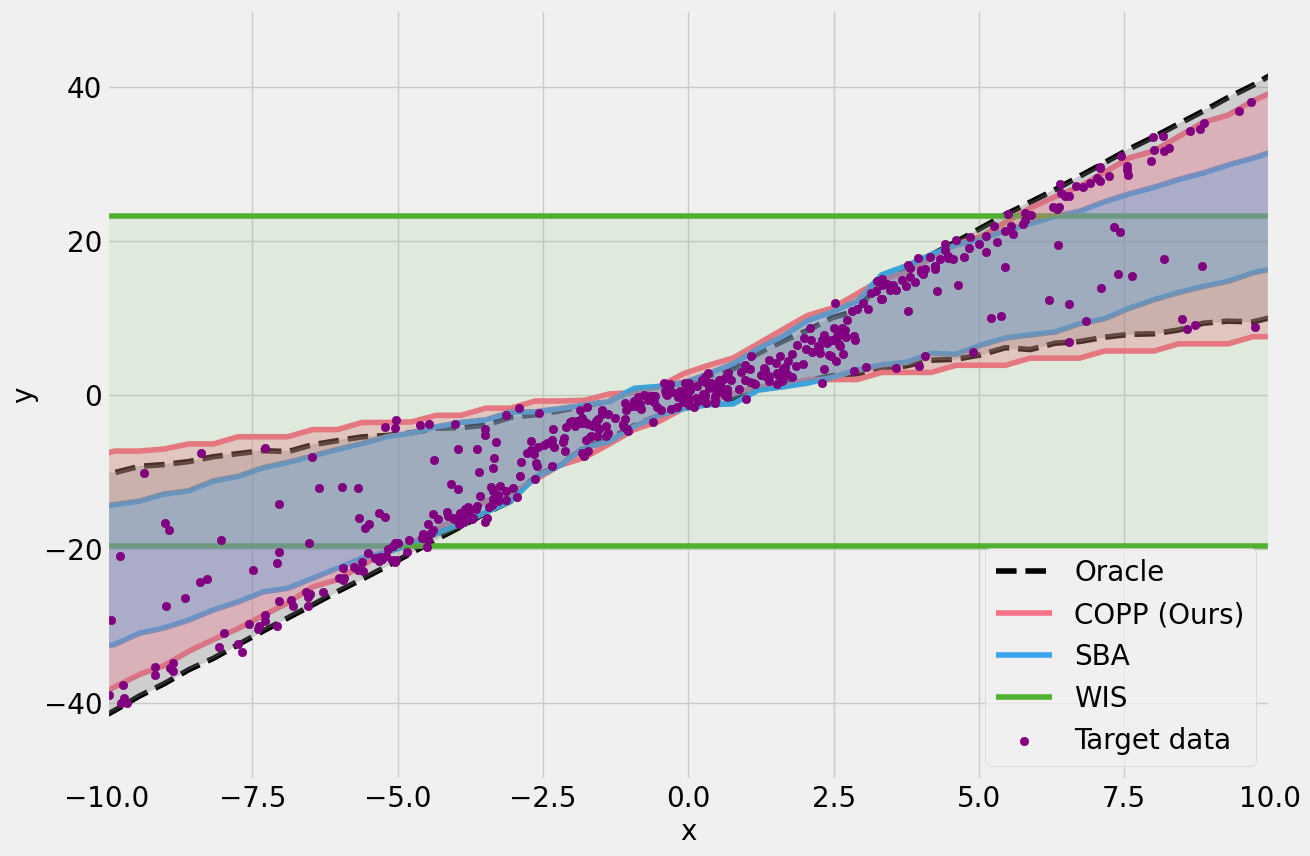
\includegraphics[width=0.50\columnwidth]{figures/copp/cis-updated.png}
%     \caption{$90\%$ predictive intervals for $Y$ as a function of $X=x$ for COPP, competing methods and the oracle.}
%     \label{fig:cis-updated}
% \end{figure}
\section{Experiments} \label{sec:exp}



\textbf{Baselines for comparison.}
Given our problem setup, there are no established baselines. Instead, we compare our proposed method COPP to the following competing methods, which were constructed to capture the uncertainty in the outcome distribution and take into account the policy shift. 
% \footnote{Link to our code has been included in a separate file}

\textbf{Weighted Importance Sampling (WIS) CDF estimator.} Given observational dataset $\mathcal{D}_{obs} = \{x_i, a_i, y_i\}_{i=1}^{n_{obs}}$, \cite{risk-assessment} proposed a non-parametric WIS-based estimator for the empirical CDF of $Y$ under $\pi^*$, 
$
\hat{F}_{WIS}(t) \coloneqq \frac{\sum_{i=1}^{n_{obs}} \hat{\rho}(a_i, x_i) \mathbbm{1}(y_i \leq t)}{\sum_{i=1}^{n_{obs}} \hat{\rho}(a_i, x_i)}
$
where $\hat{\rho}(a, x) \coloneqq \frac{\pi^*(a \mid x)}{\hat{\pi}^b(a \mid x)}$ are the importance weights. We can use $\hat{F}_{WIS}$ to get predictive intervals $[y_{\alpha/2}, y_{1-\alpha/2}]$ where $y_\beta \coloneqq \text{Quantile}_\beta(\hat{F}_{WIS})$. The intervals $[y_{\alpha/2}, y_{1-\alpha/2}]$ do not depend on $x$.



% $
% \inf_{t\in \mathbb{R}}\{t: \hat{F}_{WIS}(t) \geq \beta \}$, i.e. the quantiles of $\hat{F}_{WIS}(t)$. 

\begin{table}[t]
    \caption{Toy experiment results with required coverage $90\%$. While WIS intervals provide required coverage, the mean interval length is huge compared to COPP (see table \ref{tab:length_toy}).}
    \begin{minipage}[b]{.48\linewidth}
      \centering
      \subcaption{Mean Coverage as a function of policy shift with 2 standard errors over 10 runs.}\label{tab:coverage_toy}
      \resizebox{1\columnwidth}{!}{%
        \begin{tabular}{lccc}
\toprule
Coverage &  $\Delta_{\epsilon}=0.0$ &  $\Delta_{\epsilon}=0.1$ &  $\Delta_{\epsilon}=0.2$ \\
\midrule
COPP (Ours)            &                    \textbf{0.90 $\pm$ 0.01}&                    \textbf{0.90 $\pm$ 0.01}&                    \textbf{0.91 $\pm$ 0.01}\\
WIS                  &                    \textbf{0.89 $\pm$ 0.01}&                     \textbf{0.91 $\pm$ 0.02}&                     0.94 $\pm$ 0.02\\
SBA                  &                     \textbf{0.90 $\pm$ 0.01}&                     0.88 $\pm$ 0.01&                     0.87 $\pm$ 0.01\\
\midrule
\midrule
COPP (GT weights Ours)      &                     \textbf{0.90 $\pm$ 0.01}&                     \textbf{0.90 $\pm$ 0.01}&                     \textbf{0.90 $\pm$ 0.01}\\
CP (no policy shift) &                     \textbf{0.90 $\pm$ 0.01}&                     0.87 $\pm$ 0.01&                     0.85 $\pm$ 0.01\\
CP (union) &                      0.96 $\pm$ 0.01 &         0.96 $\pm$ 0.01 &         0.96 $\pm$ 0.01 \\
\bottomrule
\end{tabular}
}
    \end{minipage}%
    \hspace{0.5cm}
    \begin{minipage}[b]{.48\linewidth}
      \centering
      \subcaption{Mean Interval Length as a function of policy shift with 2 standard errors over 10 runs.}\label{tab:length_toy}
      \resizebox{1\columnwidth}{!}{%
        \begin{tabular}{lccc}
\toprule
Interval Lengths &  $\Delta_{\epsilon}=0.0$ &  $\Delta_{\epsilon}=0.1$ &  $\Delta_{\epsilon}=0.2$ \\
\midrule
COPP (Ours)           &                     9.08 $\pm$ 0.10&                     9.48 $\pm$ 0.22&                     9.97 $\pm$ 0.38\\
WIS                  &                    \red{24.14 $\pm$ 0.30}&               \red{32.96 $\pm$ 1.80}&             \red{43.12 $\pm$ 3.49}\\
SBA                  &                     8.78 $\pm$ 0.12&                     8.94 $\pm$ 0.10&                     8.33 $\pm$ 0.09\\
\midrule
\midrule
COPP (GT weights Ours)      &                     8.91 $\pm$ 0.09&                     9.25 $\pm$ 0.12&                     9.59 $\pm$ 0.20\\
CP (no policy shift) &                     9.00 $\pm$ 0.10&                     9.00 $\pm$ 0.10&                     9.00 $\pm$ 0.10\\
CP (union) &                     10.66 $\pm$ 0.18 &         11.04 $\pm$ 0.2 &         11.4 $\pm$ 0.26 \\
\bottomrule
\end{tabular}%
}
    \end{minipage} 
\end{table}



% \begin{table}[t!]
% \centering
% \resizebox{0.5\columnwidth}{!}{%
% \begin{tabular}{lccc}
% \toprule
% Coverage &  $\Delta_{\epsilon}=0.0$ &  $\Delta_{\epsilon}=0.1$ &  $\Delta_{\epsilon}=0.2$ \\
% \midrule
% COPP (Ours)            &                    \textbf{0.90 $\pm$ 0.01}&                    \textbf{0.90 $\pm$ 0.01}&                    \textbf{0.91 $\pm$ 0.01}\\
% WIS                  &                    \textbf{0.89 $\pm$ 0.01}&                     \textbf{0.91 $\pm$ 0.02}&                     0.94 $\pm$ 0.02\\
% SBA                  &                     \textbf{0.90 $\pm$ 0.01}&                     0.88 $\pm$ 0.01&                     0.87 $\pm$ 0.01\\
% \midrule
% \midrule
% COPP (GT weights Ours)      &                     \textbf{0.90 $\pm$ 0.01}&                     \textbf{0.90 $\pm$ 0.01}&                     \textbf{0.90 $\pm$ 0.01}\\
% CP (no policy shift) &                     \textbf{0.90 $\pm$ 0.01}&                     0.87 $\pm$ 0.01&                     0.85 $\pm$ 0.01\\
% \bottomrule
% \end{tabular}
% %
% }
% \caption{Mean Coverage as a function of policy shift with 2 standard errors over 10 runs. Required coverage is $90\%$. While WIS intervals provide required coverage, the mean interval length is huge compared to COPP (see table \ref{tab:length_toy}).}\label{tab:coverage_toy}
% \end{table}
% \begin{table}[]
% \centering
% \resizebox{0.5\columnwidth}{!}{%
% \begin{tabular}{lccc}
% \toprule
% Interval Lengths &  $\Delta_{\epsilon}=0.0$ &  $\Delta_{\epsilon}=0.1$ &  $\Delta_{\epsilon}=0.2$ \\
% \midrule
% COPP (Ours)           &                     9.08 $\pm$ 0.10&                     9.48 $\pm$ 0.22&                     9.97 $\pm$ 0.38\\
% WIS                  &                    \red{24.14 $\pm$ 0.30}&               \red{32.96 $\pm$ 1.80}&             \red{43.12 $\pm$ 3.49}\\
% SBA                  &                     8.78 $\pm$ 0.12&                     8.94 $\pm$ 0.10&                     8.33 $\pm$ 0.09\\
% \midrule
% \midrule
% COPP (GT weights Ours)      &                     8.91 $\pm$ 0.09&                     9.25 $\pm$ 0.12&                     9.59 $\pm$ 0.20\\
% CP (no policy shift) &                     9.00 $\pm$ 0.10&                     9.00 $\pm$ 0.10&                     9.00 $\pm$ 0.10\\
% \bottomrule
% \end{tabular}%
% }
% \caption{Mean Interval Length as a function of policy shift with 2 standard errors over 10 runs}\label{tab:length_toy}
% \end{table}





\textbf{Sampling Based Approach (SBA).} As mentioned in Sec. \ref{sec:weights}, we can directly use the estimated $\hat{P}(y\mid x, a)$ to construct the predictive intervals as follows. For a given $x^{test}$, we generate $A_i \overset{\textup{i.i.d.}}{\sim} \pi^*(\cdot \mid x^{test})$, and $Y_i \sim \hat{P}(\cdot \mid x^{test}, A_i)$ for $i \leq \ell$. We then define the predictive intervals for $x^{test}$ using the $\alpha/2$ and $1-\alpha/2$ quantiles of $\{Y_i\}_{i \leq \ell}$. While SBA is not a standard baseline, it is a natural comparison to make to answer the question of ``why not construct the intervals using $\hat{P}(y|x, a)$ directly''?

% In this section, we will demonstrate COPP for off-policy prediction on both, synthetic and real-world data. Due to space constraints, we have added extensive experiments on UCI datasets in \ref{sec:UCI}.

\subsection{Toy Experiment}\label{sec:exp_toy} 
 We start with synthetic experiments and an ablation study, in order to dissect and understand our proposed methodology in more detail. We assume that our policies are stationary and there is overlap between the behaviour and target policy, both of which are standard assumptions \citep{risk-assessment, drobust, ope-rl}.
\subsubsection{Synthetic data experiments setup}

In order to understand how COPP works, we construct a simple experimental setup where we can control the amount of ``\textit{policy shift}" and know the ground truth. In this experiment, $X \in \mathbb{R}$, $A \in \{1, 2, 3, 4\}$ and $Y \in \mathbb{R}$, where $X$ and $Y\mid x, a$ are normal random variables. Further details and additional experiments on continuous action spaces are given in Appendix \ref{sec:toy_experiments_descrip}.   

\textbf{Behaviour and Target Policies.}
We define a family of policies $\pi_\epsilon(a \mid x)$, where we use the parameter $\epsilon \in (0,1/3)$ to control the policy shift between target and behaviour policies. Exact form of $\pi_\epsilon(a \mid x)$ is given in \ref{sec:toy_experiments_descrip}. For the behaviour policy $\pi^b$, we use $\epsilon^b = 0.3$ (i.e. $\pi^b(a \mid x) \equiv  \pi_{0.3}(a \mid x)$), and for target policies $\pi^*$, we use $\epsilon^* \in \{0.1, 0.2, 0.3\}$. Using the true behaviour policy, $\pi^b$, we generate observational data $\mathcal{D}_{obs} = \{x_i, a_i, y_i\}_{i=1}^{n_{obs}}$ which is then split into training ($\mathcal{D}_{tr}$) and calibration ($\mathcal{D}_{cal}$) datasets, of sizes $m$ and $n$ respectively.

% \begin{figure*}[t]
%     \begin{subfigure}{0.33\textwidth}
%     \centering
%     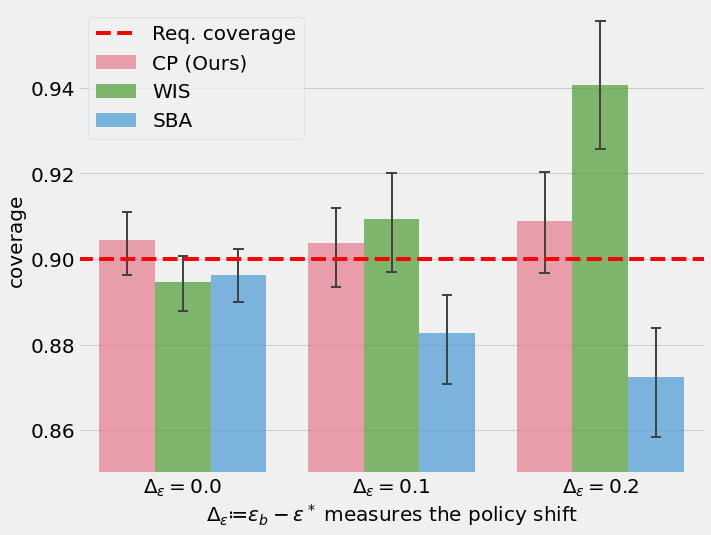
\includegraphics[height=0.8\textwidth, width=0.98\textwidth]{figures/copp/cov-pols1.png}
%     \subcaption{Coverage against policy shift}
%     \label{fig:policy-shift-toy}
%     \end{subfigure}
%     \begin{subfigure}{0.33\textwidth}
%     \centering
%     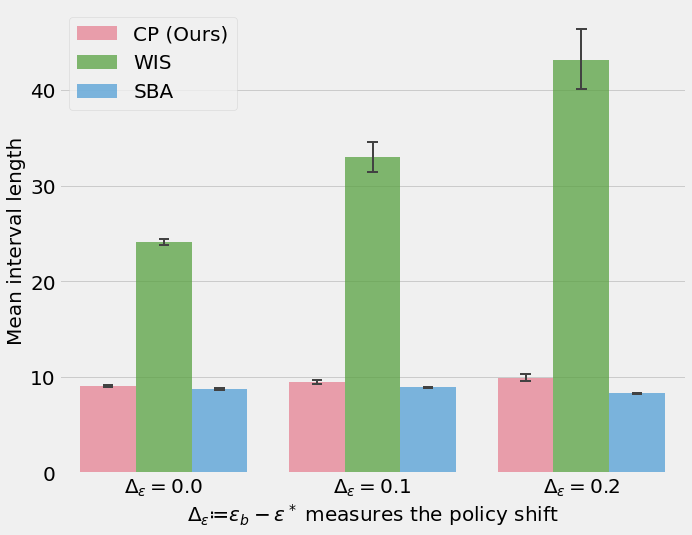
\includegraphics[height=0.8\textwidth, width=0.98\textwidth]{figures/copp/cov-pols-len1.png}
%     \subcaption{Mean Interval lengths against policy shift}
%     \label{fig:policy-shift-len}
%     \end{subfigure}
%     \begin{subfigure}{0.33\textwidth}
%     \centering
%     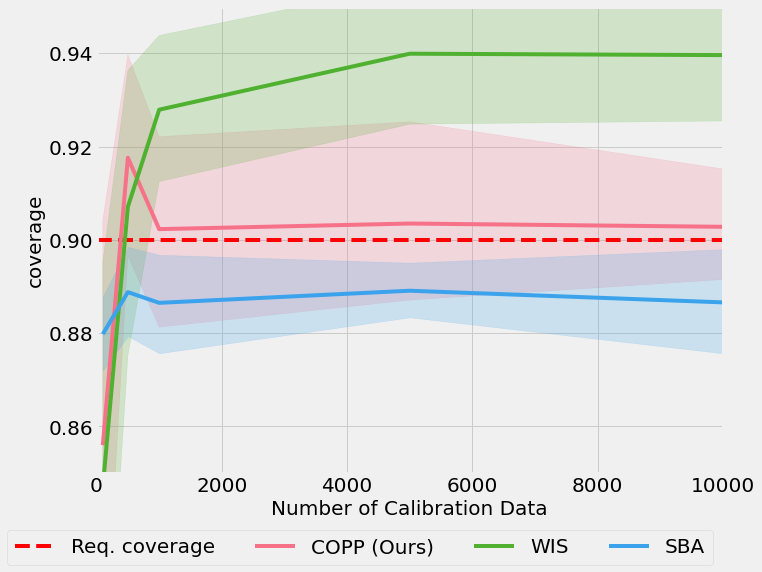
\includegraphics[height=0.8\textwidth, width=0.98\textwidth]{figures/copp/cov-n_cal.png}
%     \subcaption{Coverages against $n$}
%     \label{fig:n_cal}
%     \end{subfigure}
%     \caption{Results for synthetic data experiment with $\pi^b = \pi_{0.3}$. In figures \ref{fig:policy-shift-toy} and \ref{fig:policy-shift-len}, we consider different target policies, $\pi^* \in \{\pi_{0.1}, \pi_{0.2}, \pi_{0.3}\}$ and 5000 calibration data points. In figure \ref{fig:n_cal}, the target policy is $\pi^* = \pi_{0.1}$.}
%     \label{fig:Toy_GT}
% \end{figure*}

\textbf{Estimation of ratios, $\hat{w}(x, y)$.}
Using the training dataset $\mathcal{D}_{tr}$, we estimate $P(y | x, a)$ as $\hat{P}(y | x, a) = \mathcal{N}(\mu(x, a), \sigma(x, a))$, where $\mu(x, a), \sigma(x, a)$ are both neural networks (NNs). Similarly, we use NNs to estimate the behaviour policy $\hat{\pi}^b$ from $\mathcal{D}_{tr}$. Next, to estimate $\hat{w}(x, y)$, we use \eqref{weight-est} with $h = 500$.

\textbf{Score.}
For the score function, we use the same formulation as in \cite{romano2019conformalized}, i.e. $s(x, y) = \max\{ \hat{q}_{\alpha_{lo}}(x) - y, y - \hat{q}_{\alpha_{hi}}(x) \}$, where $\hat{q}_\beta(x)$ denotes the $\beta$ quantile estimate of $P^{\pi^b}_{Y\mid X=x}$ trained using pinball loss.

Lastly, our weights $w(x, y)$ depend on $x$ \textbf{and} $y$ and hence we use a grid of $100$ equally spaced out $y$'s in our experiments to determine the predictive interval which satisfies $\hat{C}_n(x) \coloneqq \{y: s(x,y) \leq \text{Quantile}_{1-\alpha}(\hat{F}_{n}^{x, y})\}$. This is parallelizable and hence does not add much computational overhead.

\textbf{Results.} Table \ref{tab:coverage_toy} shows the coverages of different methods as the policy shift $\Delta_{\epsilon}=\epsilon^b - \epsilon^*$ increases. The behaviour policy $\pi^b = \pi_{0.3}$ is fixed and we use $n=5000$ calibration datapoints, across 10 runs. Table \ref{tab:coverage_toy} shows, how COPP stays very close to the required coverage of $90\%$ across all target policies compared to WIS and SBA. WIS intervals are overly conservative i.e. above the required coverage, while the SBA intervals suffer from under-coverage i.e. below the required coverage. These results supports our hypothesis from Sec. \ref{sec:weights}, which stated that COPP is less sensitive to estimation errors of $\hat{P}(y|x, a)$ compared to directly using $\hat{P}(y|x, a)$ for the intervals, i.e. SBA. 

Next, Table \ref{tab:length_toy} shows the mean interval lengths and even though WIS has reasonable coverage for $\Delta_{\epsilon}=0.0$ and $0.1$, the average interval length is huge compared to COPP. Fig. \ref{fig:copp}b shows the predictive intervals for one such experiment with $\pi^* = \pi_{0.1}$ and $\pi^b = \pi_{0.3}$. We can see that SBA intervals are overly optimistic, while WIS intervals are too wide and are not adaptive w.r.t. $X$. COPP produces intervals which are much closer to the oracle intervals. 

\subsubsection{Ablation Study.} 

To isolate the effect of weight estimation error and policy shift, we conduct an ablation study, comparing COPP with estimated weights to COPP with Ground Truth (GT) weights and standard CP (assuming no policy shift). Table \ref{tab:coverage_toy} shows that at $\Delta_\epsilon = 0$, i.e. no policy shift, standard CP achieves the required coverage as expected. However the coverage of standard CP intervals decreases as the policy shift $\Delta_\epsilon$ increases. COPP, on the other hand, attains the required coverage of $90\%$, by adapting the predictive intervals with increasing policy shift. Table \ref{tab:length_toy} shows that the average interval length of COPP increases with increasing policy shift $\Delta_\epsilon$. Furthermore, Table \ref{tab:coverage_toy} illustrates that while COPP achieves the required coverage for different target policies, on average it is slightly more conservative than using COPP with GT weights. This can be explained by the estimation error in $\hat{w}(x,y)$. Additionally, to investigate the effect of integrating out the actions in \eqref{weight-est}, we also perform CP for each action $a$ separately (as in \cite{lei2020conformal}) and then take the union of the intervals across these actions. In the union method, the probability of an action being chosen is not taken into account, (i.e., intervals are independent of $\pi^*$) and hence the coverage is overly conservative as expected.


% The union method is overall too conservative, and is independent of the target policy, since the probability of an action being chosen is not taken into account when taking the union.

Lastly, we investigate how increasing the number of calibration data $n$ affects the coverage for all the methodologies. We observe that coverage of COPP is closer to the required coverage of $90\%$ compared to the competing methodologies. Additionally, the coverage of COPP converges to the required coverage as $n$ increases; see Appendix \ref{app:N-cal_exp_toy} for detailed experimental results.

% Table \ref{tab:coverage_toy}  shows that when target policy $\pi^* = \pi_{0.1}$, disregarding the policy shift leads to predictive intervals which are under-covered regardless of the number of calibration data. On the other hand, both, our methodology and CP with GT weights converges to required coverage even with 500 calibration data. One important thing to note is the smaller variance of coverage results when using GT weights, as compared to our method, as the estimation of $\hat{w}(x, y)$ adds to the variance in terms of estimation error. 
% \begin{figure*}[t]
%     \begin{subfigure}{0.33\textwidth}
%     \centering
%     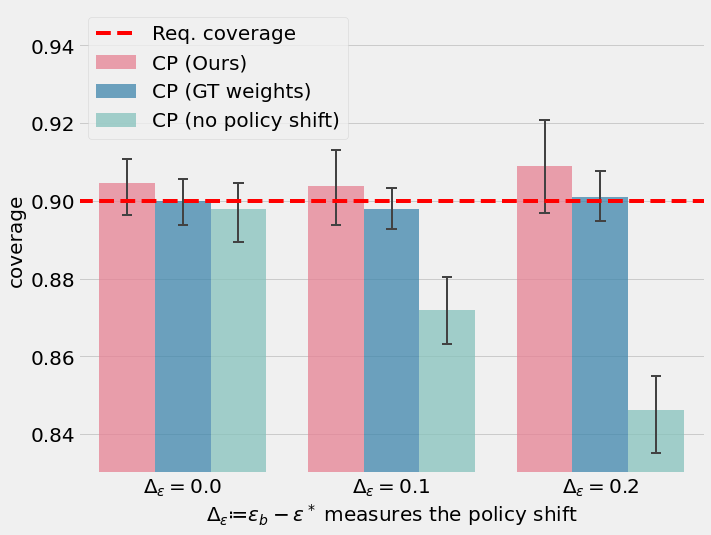
\includegraphics[height=0.8\textwidth, width=0.98\textwidth]{figures/copp/cov-pols-abl1.png}
%     \subcaption{Coverage against policy shift}
%     \label{fig:policy-shift-abl}
%     \end{subfigure}
%     \begin{subfigure}{0.33\textwidth}
%     \centering
%     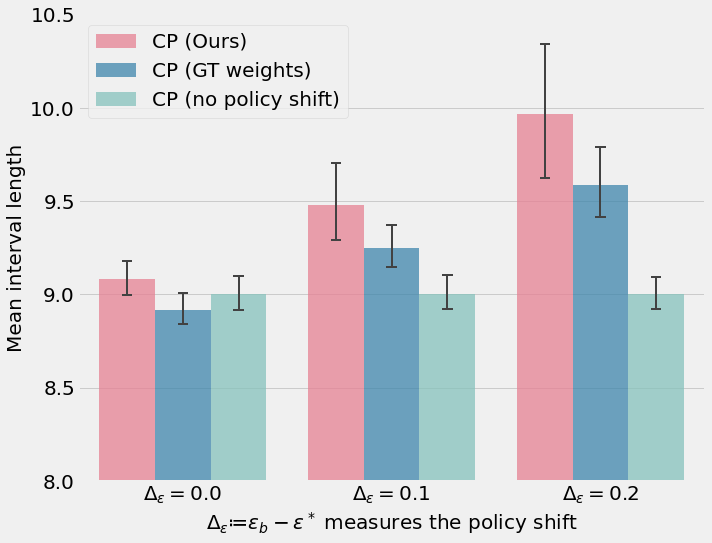
\includegraphics[height=0.8\textwidth, width=0.98\textwidth]{figures/copp/cov-lens-abl1.png}
%     \subcaption{Mean Interval lengths against policy shift} %$\pi^* \in \{\pi_{0.1}, \pi_{0.2}, \pi_{0.3}\}$}
%     \label{fig:policy-shift-len-abl}
%     \end{subfigure}
%     \begin{subfigure}{0.33\textwidth}
%     \centering
%     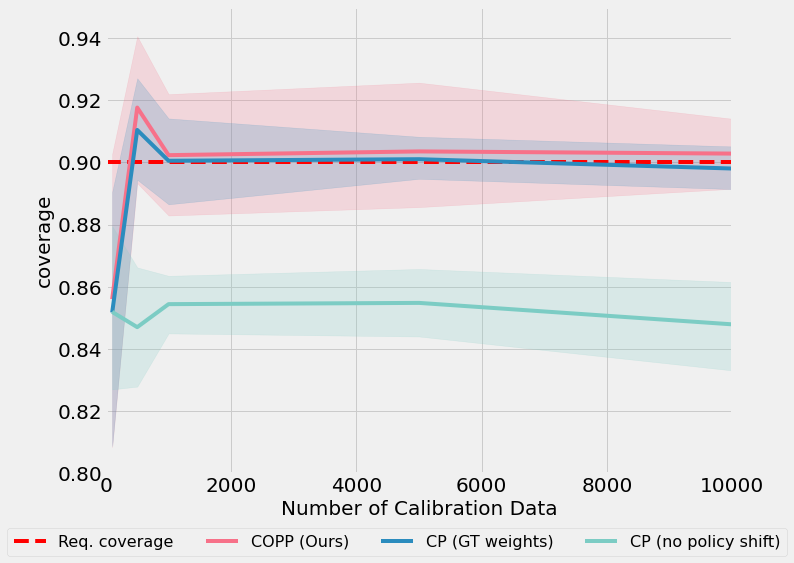
\includegraphics[height=0.8\textwidth, width=0.98\textwidth]{figures/copp/cov-n_cal-abl.png}
%     \subcaption{Coverage against $n$ with $\pi^* = \pi_{0.1}$}
%     \label{fig:ncal-abl}
%     \end{subfigure}
%     \caption{Ablation study results with $\pi^b = \pi_{0.3}$. In figures \ref{fig:policy-shift-abl} and \ref{fig:policy-shift-len-abl}, we consider different target policies, $\pi^* \in \{\pi_{0.1}, \pi_{0.2}, \pi_{0.3}\}$ and $n=5000$. In figure \ref{fig:ncal-abl}, the target policy is $\pi^* = \pi_{0.1}$.}
%     \label{fig:abl}
% \end{figure*}

\begin{table}[t]
\centering
\caption{Mean Coverage as a function of policy shift $\Delta_\epsilon$ and 2 standard errors over 10 runs. COPP attains the required coverage of $90\%$, whereas the competing methods, WIS and SBA, are over-conservative i.e. coverage above $90\%$. In addition, when we do not account for the policy shift, standard CP becomes progressively worse with increasing policy shift.}\label{tab:MSR}
\resizebox{0.7\columnwidth}{!}{%
\begin{tabular}{lccccc}
\toprule
 &  $\Delta_{\epsilon}=0.0$ &  $\Delta_{\epsilon}=0.1$ &  $\Delta_{\epsilon}=0.2$ &  $\Delta_{\epsilon}=0.3$ &  $\Delta_{\epsilon}=0.4$ \\
\midrule
COPP (Ours)            &                  \textbf{0.90 $\pm$ 0.00}&                  \textbf{0.90 $\pm$ 0.02}&                  \textbf{0.90 $\pm$ 0.01}&                  \textbf{0.89 $\pm$ 0.01}&                  \textbf{0.91 $\pm$ 0.01}\\
WIS                  &                  1.00 $\pm$ 0.00&                  1.00 $\pm$ 0.00&                  0.92 $\pm$ 0.00&                  0.94 $\pm$ 0.00&                  0.91 $\pm$ 0.00\\
SBA                  &                  0.99 $\pm$ 0.00&                  0.99 $\pm$ 0.00&                  0.98 $\pm$ 0.00&                  0.97 $\pm$ 0.00&                  0.96 $\pm$ 0.00\\
\midrule
\midrule
% CP (GT behav policy) &                  0.95 $\pm$ 0.10&                 \textbf{ 0.90 $\pm$ 0.02}&                  \textbf{0.90 $\pm$ 0.01}&                  \textbf{0.89 $\pm$ 0.01}&                  \textbf{0.91 $\pm$ 0.01}\\
CP (no policy shift) &                  \textbf{0.91 $\pm$ 0.02}&                 \textbf{ 0.92 $\pm$ 0.02}&                  0.93 $\pm$ 0.01&                  0.94 $\pm$ 0.01&                  0.96 $\pm$ 0.01\\
\bottomrule
\end{tabular}%
}
\end{table}


\subsection{Experiments on Microsoft Ranking Dataset}

We now apply COPP onto a real dataset i.e. the Microsoft Ranking dataset 30k \citep{msr, swaminathan2016off, bietti2018contextual}. Due to space constraints, we have added additional extensive experiments on UCI datasets in Appendix \ref{sec:UCI}.


\textbf{Dataset.}
% The dataset contains relevance scores for websites recommended to different users, and comprises of $30,000$ user-website pairs. For a user $i$ and website $j$, the data contains a $136$-dimensional feature vector $u_i^j$, which consists of user $i$'s attributes corresponding to website $j$, such as length of stay or number of clicks on the website. Furthermore, for each user-website pair, the dataset also contains a relevance score, i.e. how relevant the website was to the user.
The dataset contains relevance scores for websites recommended to different users, and comprises of $30,000$ user-website pairs. For each user-website pair, the data contains a $136$-dimensional feature vector, which consists of user's attributes corresponding to the website, such as length of stay or number of clicks on the website. Furthermore, for each user-website pair, the dataset also contains a relevance score, i.e. how relevant the website was to the user.

% First, given a user $i$ we sample (with replacement) $5$ websites,  $\{u_i^j\}_{j=1}^5$, from the data. Next, we reformulate this into a contextual bandit where $A \in \{1,2,3,4,5\}$ corresponds to the website we recommend to a user. For a user $i$, we define $X$ by combining the $5$ feature vectors corresponding to the user, i.e. $X \in \mathbb{R}^{5 \times 136}$, where $x_i = (u^1_{i},u^2_{i},u^3_{i},u^4_{i}, u^5_{i})$. In addition, $Y \in\{0,1,2,3,4\}$ corresponds to the relevance score for the $A$'th website, i.e. the recommended website. The goal is to construct prediction sets that are guaranteed to contain the true relevance score with a probability of $90\%$.

First, given a user, we sample (with replacement) $5$ websites from the data corresponding to that user. Next, we reformulate this into a contextual bandit where $a_i \in \{1,2,3,4,5\}$ corresponds to the action of recommending the $a_i$'th website to the user $i$. $x_i$ is obtained by combining the $5$ user-website feature vectors corresponding to the user $i$ i.e. $x_i \in \mathbb{R}^{5 \times 136}$. $y_i \in\{0,1,2,3,4\}$ corresponds to the relevance score for the $a_i$'th website, i.e. the recommended website. The goal is to construct prediction sets that are guaranteed to contain the true relevance score with a probability of $90\%$.

% This problem can be formulated as a contextual bandit by firstly, obtaining some behavioural data, where the action $A \in \{1,2,3,4,5\}$ corresponds to the website we recommend and which has been sampled from $\pi^b(a|x)$. 

% Moreover, given that we want to rank $5$ websites per user, each recommendation task will have a feature vector $X \in \mathbb{R}^{5 \times 136}$, where $x_i = (u^1_{i},u^2_{i},u^3_{i},u^4_{i}, u^5_{i})$. In addition, $Y \in\{0,1,2,3,4\}$ will correspond to the relevance score for the $A$'th website, i.e. the website that was recommended.

% We use $\hat{f}^{\textup{label}}_\theta$ to denote the relevance class predicted by $\hat{f}_\theta$, i.e. $\hat{f}^{\textup{label}}_\theta(u) \coloneqq \argmax_j\{\hat{f}_\theta(u^{j})\}$.


% \begin{align}
%     &\pi_\epsilon (a\mid X=(u^1, u^2,u^3,u^4,u^5)) \coloneqq \nonumber \\ 
%     &\epsilon \mathbbm{1}(a = \argmax_j\{ \hat{f}^{\textup{label}}_\theta(u^j \}) \nonumber \\ 
%     &+ (1-4\epsilon) \mathbbm{1}(a \neq \argmax_j\{ \hat{f}^{\textup{label}}_\theta(u^j) \}) \nonumber
% \end{align}
% The problem being considered in this dataset is somewhat analogous to the one of recommending treatment to patients in the medical setting. Specifically, in both cases we would like to recommend websites/treatments which are relevant to the users/patients and avoid ones which are not. 

\textbf{Behaviour and Target Policies.} 
We first train a NN classifier model, $\hat{f}_\theta$, mapping each 136-dimensional user-website feature vector to the softmax scores for each relevance score class. We use this trained model $\hat{f}_\theta$ to define a family of policies which pick the most relevant website as predicted by $\hat{f}_\theta$ with probability $\epsilon$ and the rest uniformly with probability $(1-\epsilon)/4$ (see Appendix \ref{sec:MSR_experiments_decrip} for more details). Like the previous experiment, we use $\epsilon$ to control the shift between behaviour and target policies. For $\pi^b$, we use $\epsilon^b = 0.5$ and for $\pi^*$, $\epsilon^* \in \{0.1, 0.2, 0.3, 0.4, 0.5\}$. 
% Using this behaviour policy $\pi^b$, we generate an observational dataset $\mathcal{D}_{obs} = \{x_i, a_i, y_i\}_{i=1}^{n_{obs}}$ which is then split into training $\mathcal{D}_{tr}$ and calibration datasets $\mathcal{D}_{cal}$, of sizes $m$ and $n$ respectively.
% We first train a NN classifier model mapping each 136-dimensional feature vector to the softmax scores for each relevance score class, $\hat{f}_\theta:\mathcal{U} \rightarrow [0,1]^5$. We use this trained model $\hat{f}_\theta$ to define a family of policies which pick the most relevant website as predicted by $\hat{f}_\theta$ with probability $\epsilon$ and the rest uniformly with probability $(1-\epsilon)/4$ (see \ref{sec:MSR_experiments_decrip} for more details). Like the previous experiment, we use $\epsilon$ to control the shift between behaviour and target policies. For $\pi^b$, we use $\epsilon^b = 0.5$ and for $\pi^*$, $\epsilon^* \in \{0.1, 0.2, 0.3, 0.4, 0.5\}$. Using this behaviour policy $\pi^b$, we generate an observational dataset $\mathcal{D}_{obs} = \{x_i, a_i, y_i\}_{i=1}^{n_{obs}}$ which is then split into training $\mathcal{D}_{tr}$ and calibration datasets $\mathcal{D}_{cal}$, of sizes $m$ and $n$ respectively.

\textbf{Estimation of ratios $\hat{w}(X, Y)$.}
To estimate the $\hat{P}(y \mid x, a)$ we use the trained model $\hat{f}_\theta$ as detailed in Appendix \ref{sec:MSR_experiments_decrip}. To estimate the behaviour policy $\hat{\pi}^b$, we train a neural network classifier model $\mathcal{X} \rightarrow \mathcal{A}$, and we use \eqref{weight-est} to estimate the weights $\hat{w}(x, y)$.
% To estimate the $\hat{P}(y \mid x, a)$ we use the trained model $\hat{f}_\theta$ as follows:
% \[
% \hat{P}(y \mid x = (u^1, u^2,u^3,u^4,u^5), a) = \hat{f}_\theta(u^a)_y
% \]
% where $\hat{f}_\theta(u^a)_y$ corresponds to the softmax prediction of $u^a$ for label $y$ under the model $\hat{f}_\theta$. To estimate the behaviour policy $\hat{\pi}^b$, we train a classifier model $\mathcal{X} \rightarrow \mathcal{A}$ using a neural network. We use \eqref{weight-est} to estimate the weights $\hat{w}(x, y)$.

\textbf{Score.} The space of outcomes $\mathcal{Y}$ in this experiment is discrete. We define $\hat{P}^{\pi^b}(y \mid x) = \sum_{i = 1}^5 \hat{\pi}^b(A = i|x) \hat{P}(y|x, A = i)$. Using similar formulation as in \cite{conf-bates}, we define the score:
$$
s(x, y) = \sum_{y' = 0}^4 \hat{P}^{\pi^b}(y' \mid x) \mathbbm{1}(\hat{P}^{\pi^b}(y' \mid x) \geq \hat{P}^{\pi^b}(y \mid x)).
$$
Since $\mathcal{Y}$ is discrete, we no longer need to construct a grid of $y$ values on which to compute $\text{Quantile}_{1-\alpha}(\hat{F}_{n}^{x, y})$. Instead, we will simply compute this quantity on each $y \in \mathcal{Y}$, when constructing the predictive sets $\hat{C}_{n}(x^{test})$.

% \begin{figure*}[t]
%     \begin{subfigure}{0.5\textwidth}
%     \centering
%     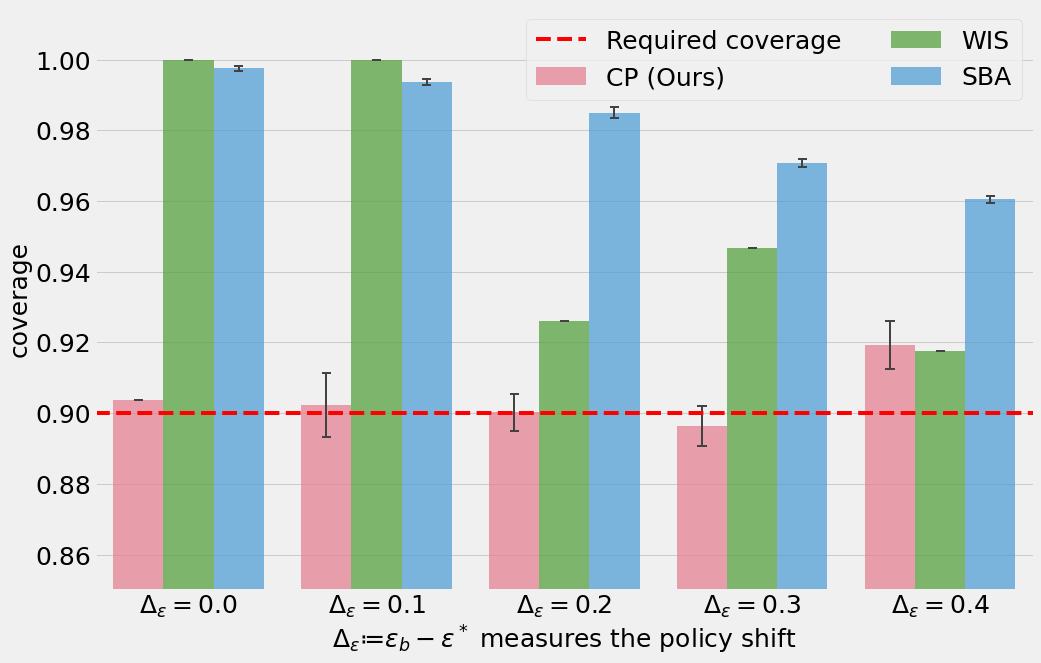
\includegraphics[height=0.6\textwidth]{figures/copp/cov-pols-msr.png}
%     \subcaption{Coverage against policy shift}
%     \label{fig:policy-shift-msr}
%     \end{subfigure}
%     \begin{subfigure}{0.5\textwidth}
%     \centering
%     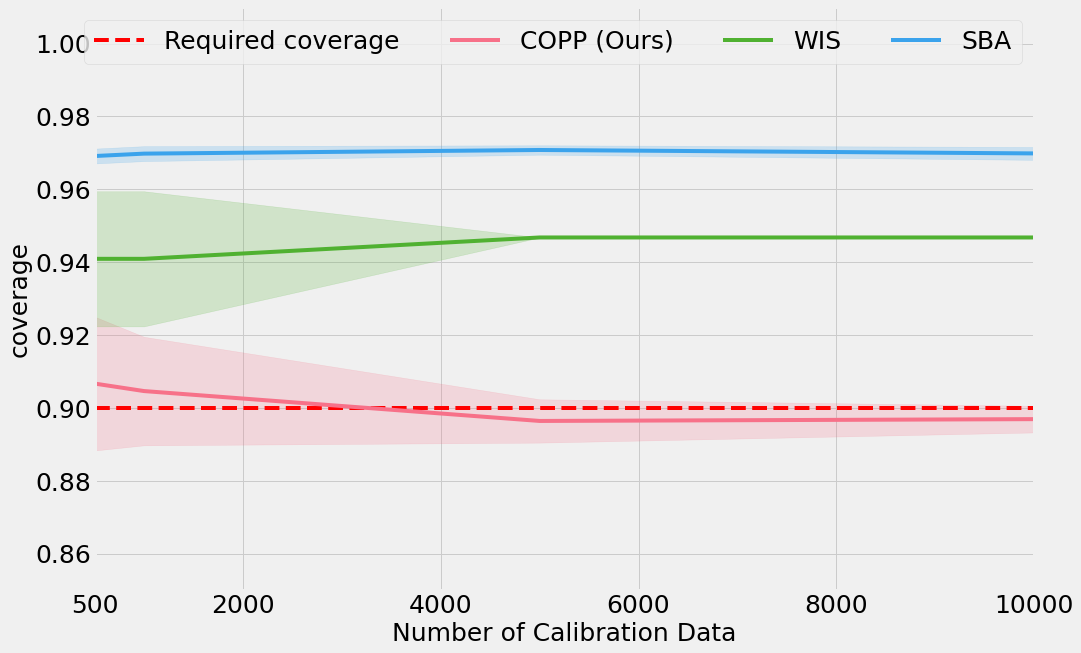
\includegraphics[height=0.6\textwidth]{figures/copp/cov-ncal-msr.png}
%     \subcaption{Coverage against $n$} %$\pi^* \in \{\pi_{0.1}, \pi_{0.2}, \pi_{0.3}\}$}
%     \label{fig:ncal-msr}
%     \end{subfigure}
%     \caption{Results of Microsoft Ranking Dataset experiment with behaviour policy $\pi^b = \pi_{0.5}$. In figure \ref{fig:policy-shift-msr}, we consider different target policies, $\pi^* \in \{\pi_{0.1}, \pi_{0.2}, \dots, \pi_{0.5} \}$ and $n=5000$. In figure \ref{fig:ncal-msr}, the target policy is $\pi^* = \pi_{0.2}$.}
%     \label{fig:msr}
% \end{figure*}

\textbf{Results.}
% Here below, we can see the coverage plots when using our proposed methods standard classification and \cite{risk-assessment}. We can see from the below plots that our proposed method is able to attain the required coverage consistently, whereas \cite{risk-assessment} is over-conservative. Lastly, if we do not use the conformal prediction framework, we can see from Fig.[ref] that we can no longer guarantee coverage and suffer from under-coverage.
Table \ref{tab:MSR} shows the coverages of different methodologies across varying target policies $\pi_{\epsilon^*}$. The behaviour policy $\pi^b = \pi_{0.5}$ is fixed and we use $n=5000$ calibration datapoints, across 10 runs. Table \ref{tab:MSR} also shows that the coverage of WIS and SBA sets is dependent upon the policy shift, with both being overly conservative across the different target policies as compared to COPP. Recall that the WIS sets do not depend on $x^{test}$ and as a result we get the same set for each test data point. This becomes even more problematic when $Y$ is discrete -- if, for each label $y$, $\tarprob(Y = y)>10\%$, then WIS sets (with the required coverage of $90\%$) are likely to contain every label $y \in \mathcal{Y}$.
% This becomes even more problematic when $Y$ is discrete as there are finitely many possible sets that can be constructed, and consequently the achieved coverage cannot be arbitrarily close to the required coverage. In particular, when $\epsilon^b=0.5$, small $\Delta_{\epsilon}$ values indicate that the target policy is well spread out with each action having at least $10\%$ probability. Hence if we would like to achieve marginal coverage of at least $90\%$, we need to include all the labels, give that the intervals are not dependent on $x$ for WIS. 
In comparison, COPP is able to stay much closer to the required coverage of $90\%$ across all target policies. We have also added standard CP without policy shift as a sanity check, and observed that the sets get increasingly conservative as the policy shift increases.

% for the target policy $\pi^* = \pi_{0.2}$ evolves 
Finally, we also plotted how the coverage changes as the number of calibration data $n$ increases. We observe again that the coverage of COPP is closer to the required coverage of $90\%$ compared to the competing methodologies. Due to space constraints, we have added the plots in Appendix \ref{app:N-cal_exp_msr}.

% Moreover, we observe that our method only requires around $500$ calibration data to obtain the required coverage, and that it converges to the required $90\%$ as the number of calibration data increases. Both, SBA and WIS on the other hand remain overly conservative even with increasing calibration data. 

% Note that we only we only included the high number of calibration data to check convergence and do not expect to have this amount of calibration data in practice.

\textbf{Class-balanced conformal prediction.}
Using the methodology described in Sec. \ref{sec:group_balanced_cov}, we construct predictive sets, $\hat{C}^{\mathcal{Y}}_n(x)$, which offer label conditioned coverage guarantees (see \ref{sec:grp-bal}), i.e. for all $y\in \mathcal{Y}$, 
$$
\tarprob(Y \in \hat{C}^{\mathcal{Y}}_n(X) \mid Y = y) \geq 1- \alpha.
$$
We empirically demonstrate that $\hat{C}^{\mathcal{Y}}_n$ provides label conditional coverage, while $\hat{C}_n$ obtained using alg. \ref{cp_covariate_shift} may not. Due to space constraints, details on construction of $\hat{C}^{\mathcal{Y}}_n$ as well as experimental results have been included in Appendix \ref{sec:results_class_bal_coverage}.

\section{Conclusion and Limitations}\label{sec:lims}

% In this paper, we construct predictive intervals for contextual bandits to assess a target policy $\pi^*$ given observational data generated from a behavioural policy $\pi^b$. 
In this paper, we propose COPP, an algorithm for constructing predictive intervals on off-policy outcomes, which are adaptive w.r.t. covariates $X$. We theoretically prove that COPP can guarantee finite-sample coverage by adapting the framework of conformal prediction to our setup.
Our experiments show that conventional methods cannot guarantee any user pre-specified coverage, whereas COPP can.
For future work, it would be interesting to apply COPP to policy training. This could be a step towards robust policy learning by optimising the worst case outcome \citep{stutz2021learning}.

We conclude by mentioning several limitations of COPP. 
Firstly, we do not guarantee conditional coverage in general.
We outline conditions under which conditional coverage holds asymptotically (Prop. \ref{conditional-res}), however, this relies on somewhat strong assumptions.
Secondly, our current method estimates the weights $w(x, y)$ through $P(y \mid x, a)$, which can be challenging.
We address this limitation in Appendix \ref{sec:alternate_weights_est}, where we propose an alternative method to estimate the weights directly, without having to model $P(y \mid x, a)$. % We leave this avenue for future work. 
Lastly, reliable estimation of our weights $\hat{w}(x, y)$ requires sufficient overlap between behaviour and target policies. The results from COPP may suffer in cases where this assumption is violated, which we illustrate empirically in Appendix \ref{subsec:cts_act}.
% We leave further consideration of how to address these limitations to future work.
We believe these limitations suggest interesting research questions that we leave to future work.

% Moreover, in this paper we have not considered the case where both the marginal in $X$ and the conditional shift, which is a straightforward extension of COPP, as the theory only relies on the ratio of the joint distribution. We leave this for future work.


\section*{Acknowledgements}
We would like to thank Andrew Jesson, Sahra Ghalebikesabi, Robert Hu, Siu Lun Chau and Tim Rudner for useful feedback.
JFT is supported by the EPSRC and MRC through the OxWaSP CDT programme (EP/L016710/1).
MFT acknowledges his PhD funding from Google DeepMind.
RC and AD are supported by the Engineering and Physical Sciences Research Council (EPSRC) through the Bayes4Health programme [Grant number EP/R018561/1].  

% \bibliographystyle{abbrv}

%%%%%%%%%%%%%%%%%%%%%%%%%%%%%%%%%%%%%%%%%%%%%%%%%%%%%%%%%%%%

\begin{comment}


\section*{Checklist}


%%% BEGIN INSTRUCTIONS %%%
% The checklist follows the references.  Please
% read the checklist guidelines carefully for information on how to answer these
% questions.  For each question, change the default \answerTODO{} to \answerYes{},
% \answerNo{}, or \answerNA{}.  You are strongly encouraged to include a {\bf
% justification to your answer}, either by referencing the appropriate section of
% your paper or providing a brief inline description.  For example:
% \begin{itemize}
%   \item Did you include the license to the code and datasets? \answerYes{See Section~\ref{gen_inst}.}
%   \item Did you include the license to the code and datasets? \answerNo{The code and the data are proprietary.}
%   \item Did you include the license to the code and datasets? \answerNA{}
% \end{itemize}
% Please do not modify the questions and only use the provided macros for your
% answers.  Note that the Checklist section does not count towards the page
% limit.  In your paper, please delete this instructions block and only keep the
% Checklist section heading above along with the questions/answers below.
%%% END INSTRUCTIONS %%%


\begin{enumerate}


\item For all authors...
\begin{enumerate}
  \item Do the main claims made in the abstract and introduction accurately reflect the paper's contributions and scope?
    \answerYes{}
  \item Did you describe the limitations of your work?
    \answerYes{} See section \ref{sec:lims}.
  \item Did you discuss any potential negative societal impacts of your work?
    \answerNA{}
  \item Have you read the ethics review guidelines and ensured that your paper conforms to them?
    \answerYes{}
\end{enumerate}


\item If you are including theoretical results...
\begin{enumerate}
  \item Did you state the full set of assumptions of all theoretical results?
    \answerYes{} See section \ref{sec:theory}.
        \item Did you include complete proofs of all theoretical results?
    \answerYes{} See section \ref{sec:proofs}.
\end{enumerate}


\item If you ran experiments...
\begin{enumerate}
  \item Did you include the code, data, and instructions needed to reproduce the main experimental results (either in the supplemental material or as a URL)?
    \answerYes{} See section \ref{sec:exps_app}.
  \item Did you specify all the training details (e.g., data splits, hyperparameters, how they were chosen)?
    \answerYes{} See sections \ref{sec:exp}, \ref{sec:exps_app}.
        \item Did you report error bars (e.g., with respect to the random seed after running experiments multiple times)?
    \answerYes{} See sections \ref{sec:exp}, \ref{sec:exps_app}.
        \item Did you include the total amount of compute and the type of resources used (e.g., type of GPUs, internal cluster, or cloud provider)?
    \answerYes{}See section \ref{sec:exps_app}.
\end{enumerate}


\item If you are using existing assets (e.g., code, data, models) or curating/releasing new assets...
\begin{enumerate}
  \item If your work uses existing assets, did you cite the creators?
    \answerNA{}
  \item Did you mention the license of the assets?
    \answerNA{}
  \item Did you include any new assets either in the supplemental material or as a URL?
    \answerNA{}
  \item Did you discuss whether and how consent was obtained from people whose data you're using/curating?
    \answerNA{}
  \item Did you discuss whether the data you are using/curating contains personally identifiable information or offensive content?
    \answerNA{}
\end{enumerate}


\item If you used crowdsourcing or conducted research with human subjects...
\begin{enumerate}
  \item Did you include the full text of instructions given to participants and screenshots, if applicable?
    \answerNA{}
  \item Did you describe any potential participant risks, with links to Institutional Review Board (IRB) approvals, if applicable?
    \answerNA{}
  \item Did you include the estimated hourly wage paid to participants and the total amount spent on participant compensation?
    \answerNA{}
\end{enumerate}


\end{enumerate}
\end{comment}

%%%%%%%%%%%%%%%%%%%%%%%%%%%%%%%%%%%%%%%%%%%%%%%%%%%%%%%%%%%%
\newpage

